\chapter{Visual Studio} \label{ch:VS}

    \FloatBarrier
    \section{Installing Visual Studio}

The first thing we are going to do is to install the latest version of Visual Studio, the IDE, in our computer. We have to \textbf{download the installer} of the program in the tab \textit{Downloads} of the official website (\url{https://visualstudio.microsoft.com/es/downloads/}). There, Microsoft offers the installers for the Community, Professional and Enterprise versions\footnote{In the same webpage Microsoft give us the possibility of downloading another tool: Visual Studio Code. In the introduction of this guide we explain why we use Visual Studio instead of this editor.}. Please notice that Professional and Enterprise releases have to be paid in case no license is obtained. However, the Community version is free and it is enough in most of the cases for the use we are going to make. If you are interested in the \textbf{VS Enterprise distribution} see how to install it with an academic license in the section \ref{sec:Enterprise}.

\begin{IN}
    \begin{itemize}
        \item Please notice that Visual Studio \textbf{MUST be installed in the first place}. The compilers, interpreters and extensions needed will be included later and with them all the tools that ensures the compatibility with all releases of Visual Studio installed in the computer.
        \item The examples of this book are created using Visual Studio 2017 and 2019. Typically, the Microsoft webpage offers the latest version of the IDE, however, you will find a previous distribution to download in case your computer is running an older Windows version (like Windows 8 for example).
    \end{itemize}
\end{IN}

When opening the url we quickly find the section reserved for the last release of Visual Studio (see Figure \ref{fig:VisualDownload}). In case the Visual Studio downloads are not shown, we can look for it by scrolling down the webpage or writing ``Microsoft Visual Studio'' in the space reserved for the search of downloads. We can obtain the installer of the Community version by clicking on \textit{Free Download }in that distribution.  A file is downloaded on our computer, the name should be something similar to \texttt{vs\_yyyyyyyy\_xxxxx.exe} where the distribution appears instead of ``y'' and a number of version appears in the place of the ``x''. We have chosen the Community version so we obtain a file similar to \texttt{vs\_community\_\_2074385403.1558468341.exe}. In case a more complete IDE version is needed, later it is explained how to obtain a student license and download the Enterprise distribution of the tool.

\begin{figure}
    \centering
    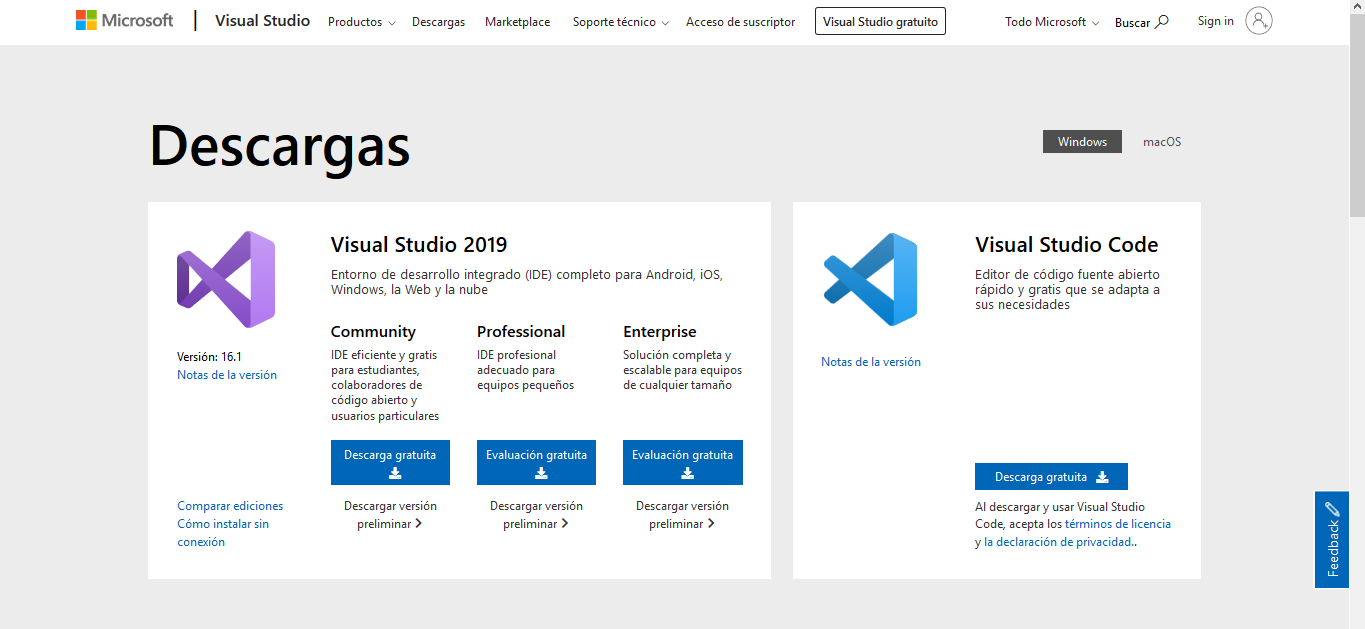
\includegraphics[width= \textwidth]{Figures/VisualDownload}
    \caption{Downloads tab of Microsoft Visual Studio webpage where the different installers for the distributions available can be downloaded.}
    \label{fig:VisualDownload}
\end{figure}

\newpage
Installing Visual Studio Community version:

\begin{enumerate}
    
    \item Execute the installer you have obtained. Accept first that the execution is done as an administrator and later accept the privacy conditions and the terms of the license of the software by clicking on \textit{Continue}. Wait for the program to download and start installing (see Figures \ref{fig:Instalacion-1} and \ref{fig:Instalacion0}).
    
    \item When finished, some options will appear in a window. There are four different tabs: Workloads, Individual Components, Language Packages and Installation folder. This tool called Visual Installer is essential for obtaining compilers and other tools used with different programming languages. In Workloads we choose \textit{Desarrollo para el escritorio con C++} and in Language Packages we choose: English or both Spanish and English (see figure \ref{fig:Instalacion1}).
    
    \item Click on \textit{Install} and wait (it might be slow).
    
    \item Once finished close all windows and restart the computer.
    
%    \item Execute Visual Studio. The first time some welcome windows appear (see figure \ref{fig:Instalacion2}), first we are going to Start Session. Although Community distribution is free for the people we first obtain a license for 30 days. In order to activate the product we have to initiate session. Click on Initiate Session. In the window that appears use your institutional email (finished with \textit{@alumnos.upm.es}), you will be redirected to the organization's sign-in page of the UPM. There you have to write again the same email and the password for that account and confirm the process. A webpage with the header ``Servicio de Identidad de RedIRIS'' may appear.
    \item Execute Visual Studio. The first time some welcome windows appear (see figure \ref{fig:Instalacion2}), first we are going to Start Session. Although Community distribution is free for the people we first obtain a license for 30 days and we have to initiate session in order to activate the product. Click on Initiate Session and in the new window that appears use your Microsoft account or your institutional email\footnote{If you use the institutional email of the UPM (finished with \textit{@alumnos.upm.es}), you will be redirected to the organization's sign-in page of the UPM. There you have to write again the same email and the password for that account and confirm the process. A webpage with the header ``Servicio de Identidad de RedIRIS'' may appear.}, in case you do not have a Microsoft account create it using the available link: \textit{Create one!}.
    
    \item Now the IDE starts to configure everything so it can take awhile. An Start window appears but you can click on \textit{Continue without code} and you access directly to the environment.
    
%    \item Notice that in the top right part of the IDE it is shown that you have already started session. If you click on the letter of your name and ``Account Configuration'' (see figure \ref{fig:Instalacion3}) you will see that your credentials are activated. In the right part of that window it may say that you are using a 30 days license, click on ``Search for an updated license'' and it automatically activate the product since you are using a personal session (see figure \ref{fig:Instalacion4}). 
    \item Now you have to check if the product is already activated with a license. Notice that the initial of your name appears in the top right part of the IDE so you have already started session. If you click on the letter of your name and \textit{Account Configuration} (see figure \ref{fig:Instalacion3}) you will see that your credentials are activated. In the right part of that window it may say that you are using a 30 days license, click on \textit{Search for an updated license} and it automatically activates the product (see figure \ref{fig:Instalacion4}).
    
    \item Your IDE is ready to work now. 
    
\end{enumerate}

\begin{figure}
    \centering
    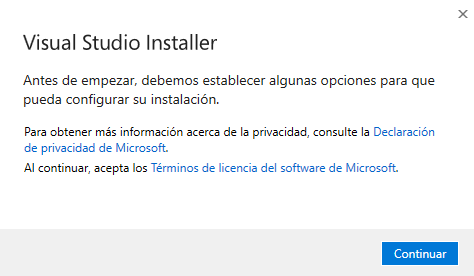
\includegraphics[width=  \textwidth]{Figures/Instalacion-1}
    \caption{First window that appears when executing the Visual Studio installer.}
    \label{fig:Instalacion-1}
\end{figure}

\begin{figure}
    \centering
    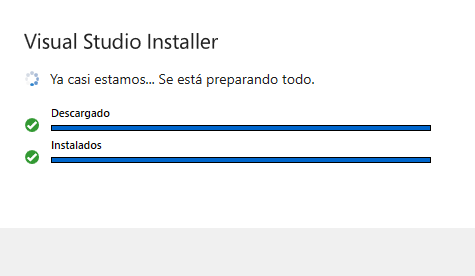
\includegraphics[width= \textwidth]{Figures/Instalacion0}
    \caption{Download and installation process of the Visual Studio environment.}
    \label{fig:Instalacion0}
\end{figure}

\begin{figure}
    \centering
    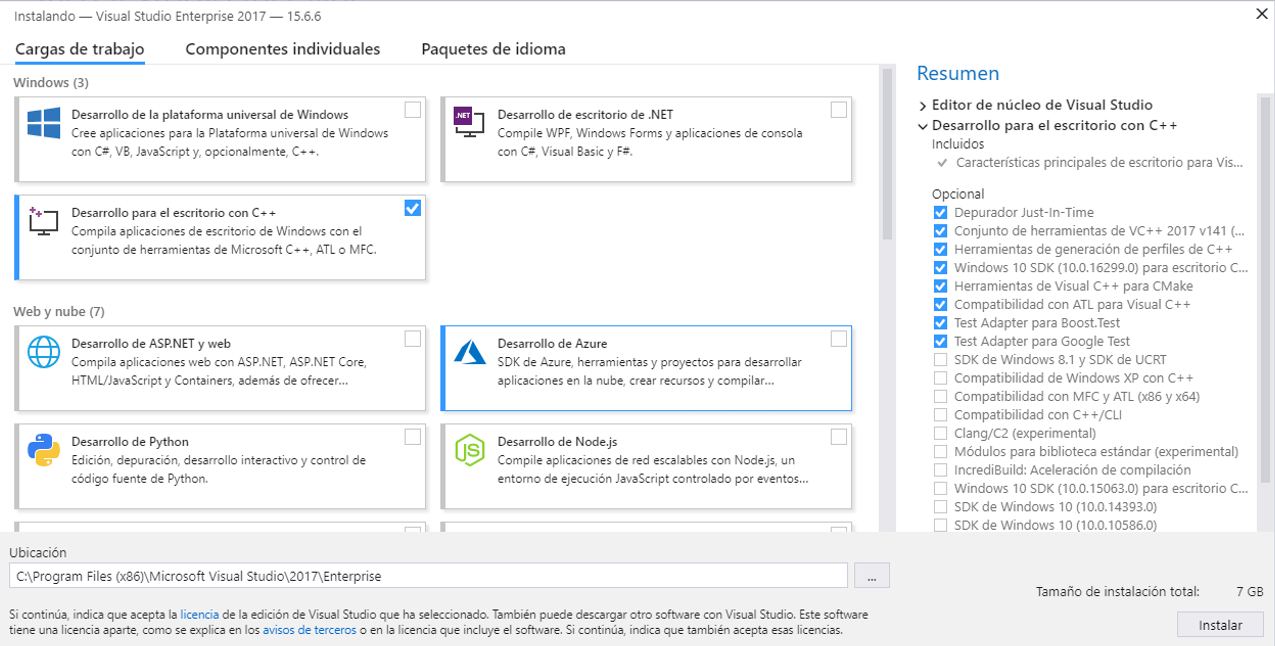
\includegraphics[width= \textwidth]{Figures/Instalacion1}
    \caption{Workload to be chosen in the installation process, \textit{desarrollo para el escritorio con C++} is selected in this step. In language package we choose at least English.}
    \label{fig:Instalacion1}
\end{figure}

\begin{figure}
    \centering
    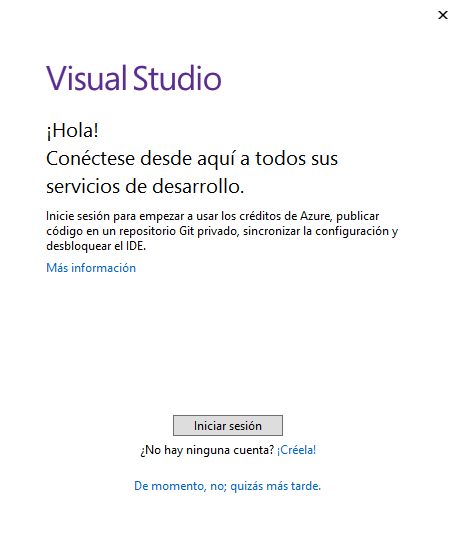
\includegraphics[width=0.7 \textwidth]{Figures/Instalacion2}
    \caption{Start window that appears after the installation, we have to start session now in order to use the options of Community version with no limit.}
    \label{fig:Instalacion2}
\end{figure}

\begin{figure}
    \centering
    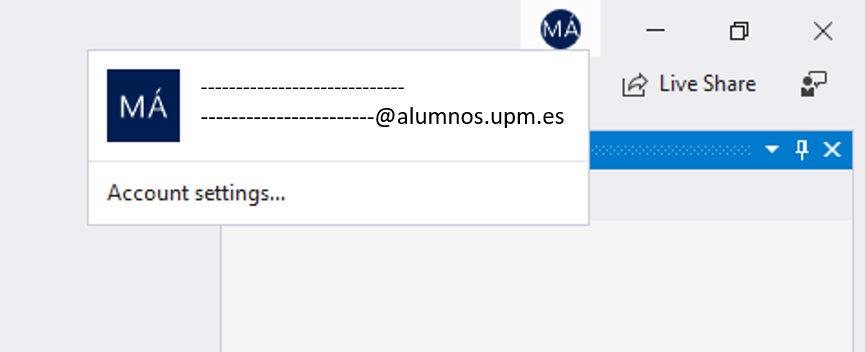
\includegraphics[width= \textwidth]{Figures/Instalacion3}
    \caption{Account Configuration inside the IDE, here we can activate the license and manage our accounts. You can use an institutional email or the Microsoft account.}
    \label{fig:Instalacion3}
\end{figure}

\begin{figure}
    \centering
    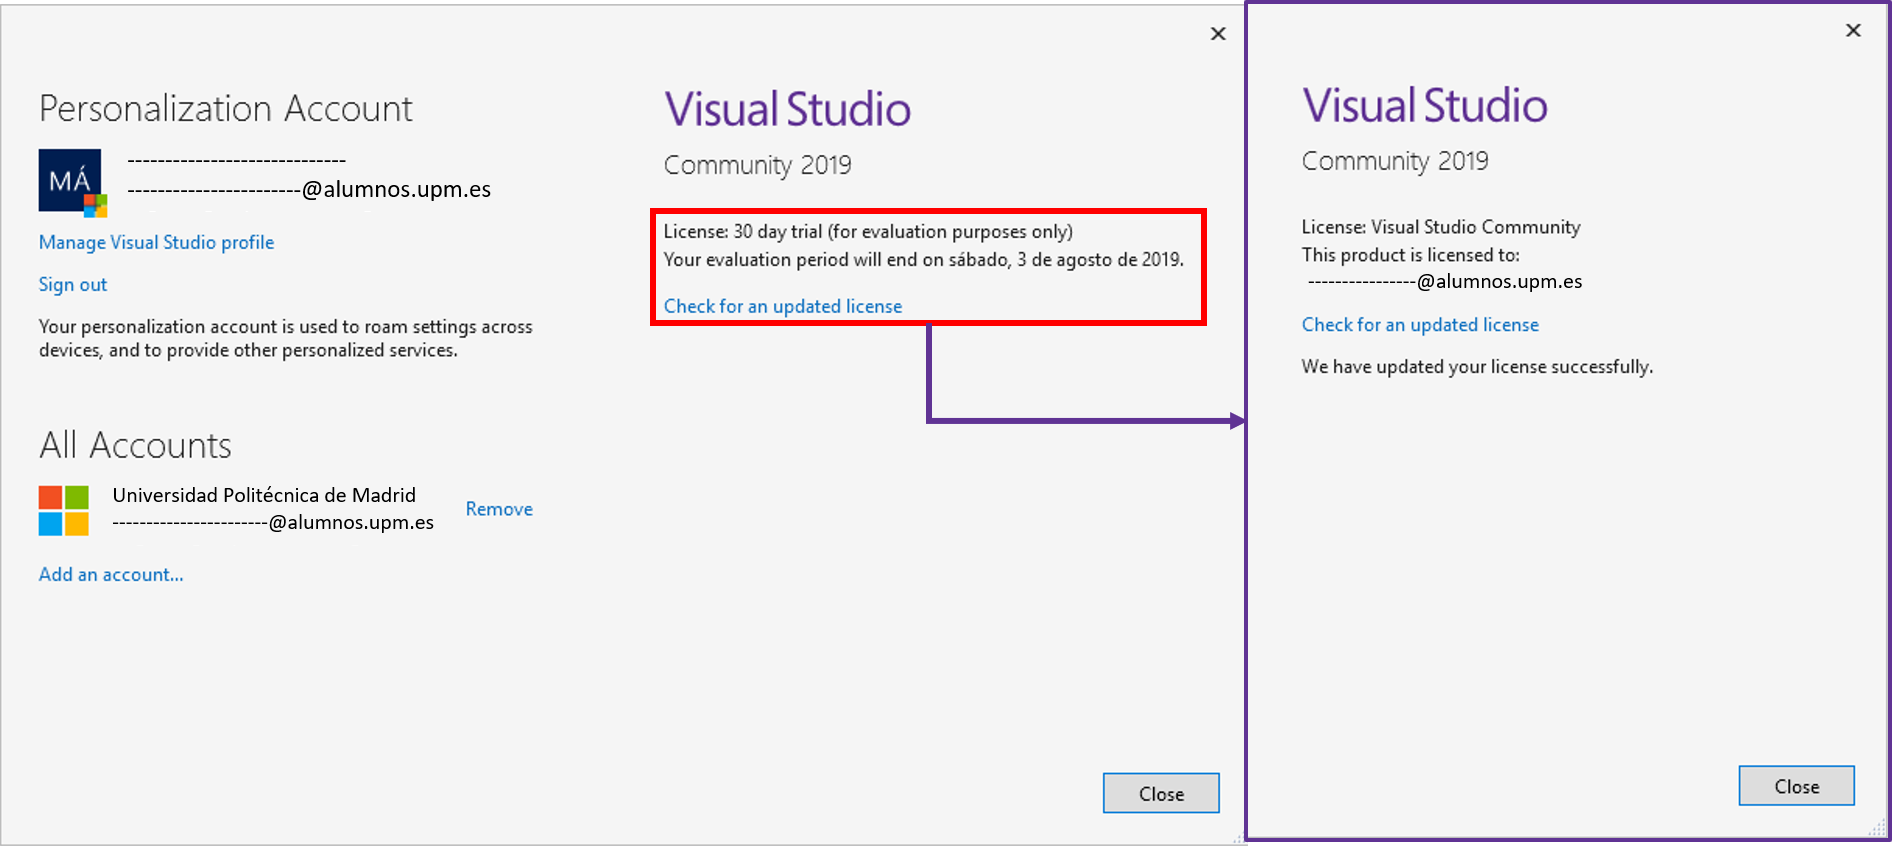
\includegraphics[width= \textwidth]{Figures/Instalacion4}
    \caption{Account Configuration menu, click on \textit{Search for an updated license} if your product is not already activated.}
    \label{fig:Instalacion4}
\end{figure}


Together with the environment itself, the \textbf{Visual Studio Installer} has been included in our computer, we can check it in the Start menu of Windows. We have seen this tool before during the process (Figure \ref{fig:Instalacion1}) and we are going to open it a few more times if we install all the programming languages and tools explained in this guide. For example, all the necessary tools needed for writing Cordova projects (smartphone applications) or the minimum templates used in a basic webpage can be installed using this installer.

It is interesting to become familiarized with the different ways of installing new functionalities, tools, extensions and updates in this IDE. First of all, we can use the \textbf{Visual Studio Installer} which can be opened through Windows OS using its shortcut as an administrator and also through the IDE by clicking on \textit{Tools/Get Tools and Features...}. Both ways show us the workloads that are already installed and the new functionalities available. We can also click on \textbf{\textit{Tools/Extensions and Updates...}} and navigate through the big amount of complements that appears. For example, the Arduino tool that is provided by \textit{Visual Micro} in order to write, upload, debug Arduino programs or burn microcontrollers with Visual Studio can be installed using this window. Finally, some programming languages like Python needs from the \textbf{installation of packages}, a topic that is treated further in the section \ref{sec:Python}.

\begin{IN}
    \begin{itemize}
        \item You are going to create a lot of projects in Visual Studio from now on. Even though the menu for creating projects is in the same place for all the programming languages (\textit{File/New/Project...}), we have noticed that the window that appears in the different versions of the IDE (2017 vs 2019 for example) differs. The fields to fill and the name of the available projects are the same but the menu is different; in Visual Studio 2017 you will find something like Figure \ref{fig:Pro2} while in the 2019 version something like Figure \ref{fig:C++1}.
        
        \item The Visual Studio installer has to be periodically updated. If you are going to install anything with the VS installer and a message appears when opening the tool, do not doubt in updating it by clicking on the pertinent option. Once finished you can resume the installation process. 
    \end{itemize}
\end{IN}


    \FloatBarrier
    \section{Configuring Visual Studio features} \label{sec:ConfigVS}

Now we are going to look through a list of useful functions and general common features that Visual Studio offers. All of them, when controlled, make the process of programming simpler:

\begin{enumerate}[nosep]
    \item Language
    \item Line numbers
    \item Navigation through files
    \item Look for references
    \item Open the definition of source functions and variables
    \item Show description of intrinsic and new functions
    \item Executing the program: \textit{Start without Debugging}
    \item Outlining blocks
    \item Additional requirements
    \item Common IDE configuration
    \item Windows inside the IDE
    \item Find in Files, Find and Replace
\end{enumerate}

\begin{enumerate}
	%%%%%%%%%%%%%%%%%%%%%%%%%%%%%%%%%%%%%%%%%%%%%%%%%%%%%%%%%%%%%%%%%%%%%%%%%%%%%%%%%C
	\item \textbf{Language}
	
	This manual has been written assuming that the IDE is configured in English, if you have used Spanish as default language, it can be changed in \textit{Tools/Options/International Settings}. There are options and commands with no intuitive translation to Spanish so we recommend getting used to the English version of the IDE and the English name of the programming concepts.
	
    
	%%%%%%%%%%%%%%%%%%%%%%%%%%%%%%%%%%%%%%%%%%%%%%%%%%%%%%%%%%%%%%%%%%%%%%%%%%%%%%%%%C
	\item \textbf{Line numbers} 
	
    %	Why showing line numbers is useful can be clear, but there are good practices that appear when our code is going to be shown in a text document (\LaTeX). It is useful to write before some subroutines, functions or other pieces of code a comment with the line number itself. For example, if our subroutine starts in the line 345, we can write a comment in that line saying ``this is the line 345''. Hence, the code is ``fixed'' in that position. We must not move it when expanding the program so it is interesting to reserve some space before and after every subroutine and function in case new lines have to be added. When writing documentation about our code in \LaTeX, it looks for the code and extracts some lines and the specific part of the program will always be in the same position among all the program.
    The line numbers are unique assignments for each of the code lines of your program (see Figure \ref{fig:LineNumbers}). This essential tool is used in all the programming languages mentioned in this guide, they are specially helpful when a list of errors appears in the compilation and each error must be found (in a specific file and line) in order to fix them. It is a good idea to change the configuration of the IDE to show them by default, independently of the language. Go to \textit{Tools/Options...} and in the menu \textit{Text Editor/All Languages/General} select the option \textit{Line numbers}. These numbers are also an easy way of referencing your code in case of writing documentation about it. 
    
    \begin{figure}
        \centering
        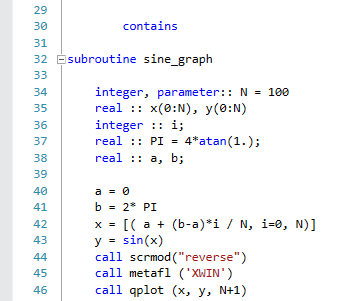
\includegraphics[width=0.7\textwidth]{Figures/LineNumbers}
        \caption{Example of the line numbers that leads all the code lines of a program.}
        \label{fig:LineNumbers}
    \end{figure}
	
	
    \newpage
	%%%%%%%%%%%%%%%%%%%%%%%%%%%%%%%%%%%%%%%%%%%%%%%%%%%%%%%%%%%%%%%%%%%%%%%%%%%%%%%%%C
	\item \textbf{Navigation through files}
	
	There are some basic functionalities that are very useful when managing big codes. The following features are activated by default in the IDE and both simplify the navigation across files. %others should be set in the configuration of Visual.
    
    \textbf{Navigation buttons:} \textit{Navigate Backward} and \textit{Navigate Forward} (Figure \ref{fig:Commands2}) have the same roles as Back and Forward in Windows OS but, instead of navigate across folders, we navigate across our opened and recently viewed codes.
    
    \begin{figure}
        \centering
        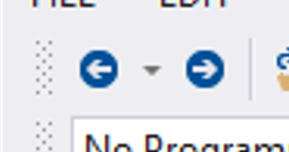
\includegraphics[width= 0.3 \textwidth]{Figures/Commands2}
        \caption{Navigation buttons: \textit{Navigate Backward} and \textit{Navigate Forward}.}
        \label{fig:Commands2}
    \end{figure}
    
    
    %%%%%%%%%%%%%%%%%%%%%%%%%%%%%%%%%%%%%%%%%%%%%%%%%%%%%%%%%%%%%%%%%%%%%%%%%%%%%%%%%C
    \item \textbf{Look for references}
    
    Even more powerful tools when we navigate through codes are \textit{Go To Definition} and \textit{Find All References}. In order to enable the possibility of looking for all references, we click on \textit{Tools/Options.../Text Editor/Fortran/Advanced} and we select \textit{True} in the option \textit{Enable Find All References} (as can be seen in the Figure \ref{fig:Commands3}).
    
    \textbf{Find All References} function, as the name says, will look for the text we want in the whole project. If it is a variable, we can know how many times (and where) is used, changed, printed, etc. and if it is a subroutine we can find where is called and where is defined. In order to use it we have to click with the right button in the name of the element and click in this option.
    
    \begin{figure}
        \centering
        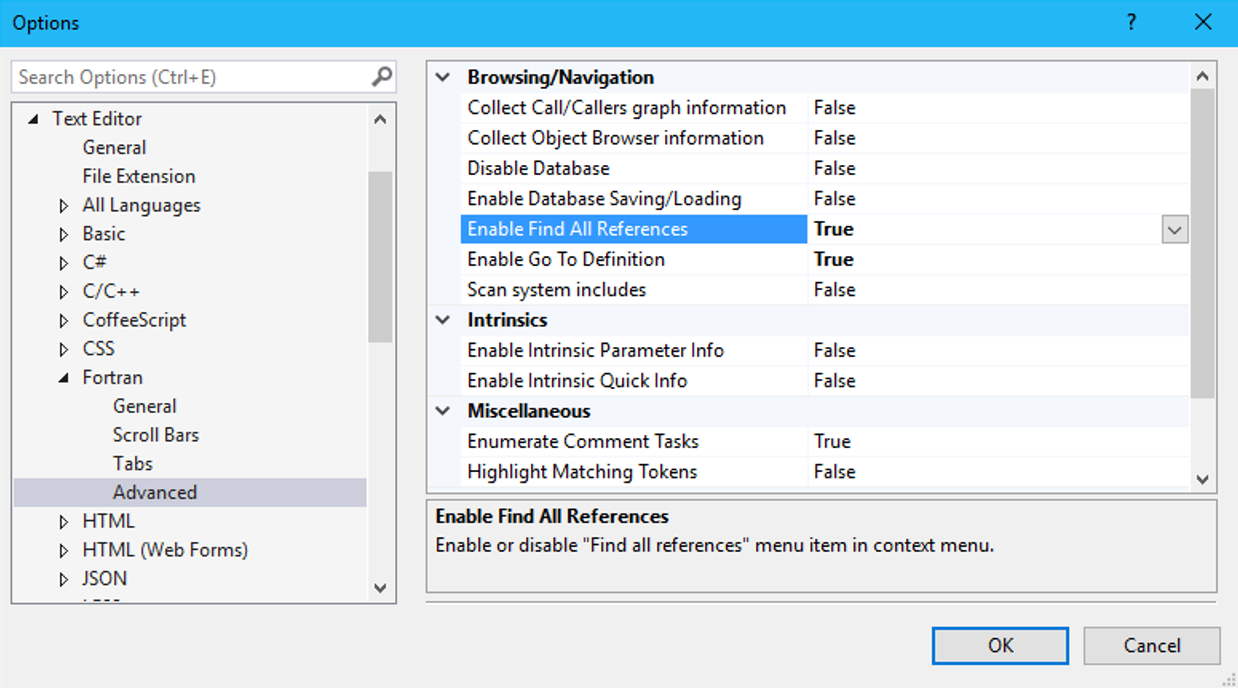
\includegraphics[width= \textwidth]{Figures/Commands3}
        \caption{\textit{Enable Find All References} and \textit{Enable Go To Definition} options to activate in the Visual Studio configuration.}
        \label{fig:Commands3}
    \end{figure}
    
    \begin{IN}
        Notice that Visual Studio has a very useful search engine that can be accessed with toolbars. The command needed is \textit{Find in files} or just \textit{Find} and it can also be minimised and put everywhere in the screen, ready to be used whenever. It is treated later in the item \ref{list:FIND}.
    \end{IN}
    
    \newpage
    %%%%%%%%%%%%%%%%%%%%%%%%%%%%%%%%%%%%%%%%%%%%%%%%%%%%%%%%%%%%%%%%%%%%%%%%%%%%%%%%%C
    \item \textbf{Open the definition of source functions and variables}
    
    Exactly like the previous tool, \textit{Go to Definition} function have to be enabled in \textit{Tools/Options.../Text Editor/Fortran/Advanced} and selecting \textit{True} in the option \textit{Enable Go To Definition} (see the Figure \ref{fig:Commands3}).
    
	\textbf{Go to Definition} function allows us to find the declaration of any variable in our code. If we for example manage a big program with multiple files and we do not know the meaning of a variable, we can click with the right button of our mouse in the variable and select this option. The window automatically moves to the line where the variable is declared, whether it is in the same file or in a different one (opening then the specific module or file with the declaration). If this tool is used with a subroutine or function, a different file will also be opened in a new window, showing then the definition of the requested piece of code. It is important to notice that, for example in the case of Fortran, it does not work if the subroutine is in a module or library already compiled but if we have included the source code in our project, we will be able to navigate quickly through files.
    
    
	%%%%%%%%%%%%%%%%%%%%%%%%%%%%%%%%%%%%%%%%%%%%%%%%%%%%%%%%%%%%%%%%%%%%%%%%%%%%%%%%%C
    \item \textbf{Show description of intrinsic and new functions}
	
	\textit{Enable Intrinsic Parameter Info} and \textit{Enable Intrinsic Quick Info} make faster the writing of code, both show quick information about functions and subroutines dynamically. To activate these features go to the menu \textit{Tools/Options.../Text Editor/Fortran/Advanced} and mark \textit{True} in the mentioned names (see Figure \ref{fig:Commands4}). The first one, \textbf{Enable Intrinsic Parameter Info}, ``\textit{displays the signature of an intrinsic in a tooltip when a user types the parameter list start character}''. This means that some essential information about the procedures and arguments will appear when typing a parenthesis after an intrinsic function or subroutine. The Figure \ref{fig:Commands5} shows an example with the cosine function. The second option, \textbf{Enable Intrinsic Quick Info}, displays intrinsic information and descriptions when we place the pointer over an intrinsic name. In the Figure \ref{fig:Commands6}, for example, a list of arguments associated to the subroutine is shown when the pointer stays on the function \texttt{Wave\_equation\_2D}.
	
	\begin{figure}
		\centering
		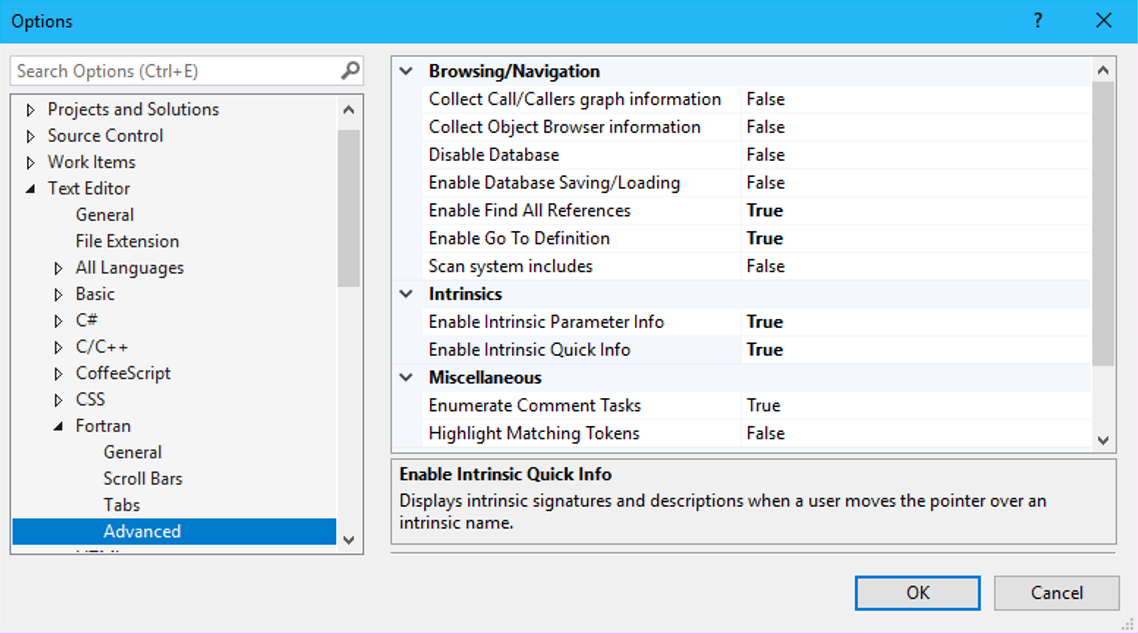
\includegraphics[width=  \textwidth]{Figures/Commands4}
		\caption{\textit{Enable Intrinsic Parameter Info} and \textit{Enable Intrinsic Quick Info} are both really useful when our codes become long and they are spread in multiple source files.}
		\label{fig:Commands4}
	\end{figure}
	
	\begin{figure}
		\centering
		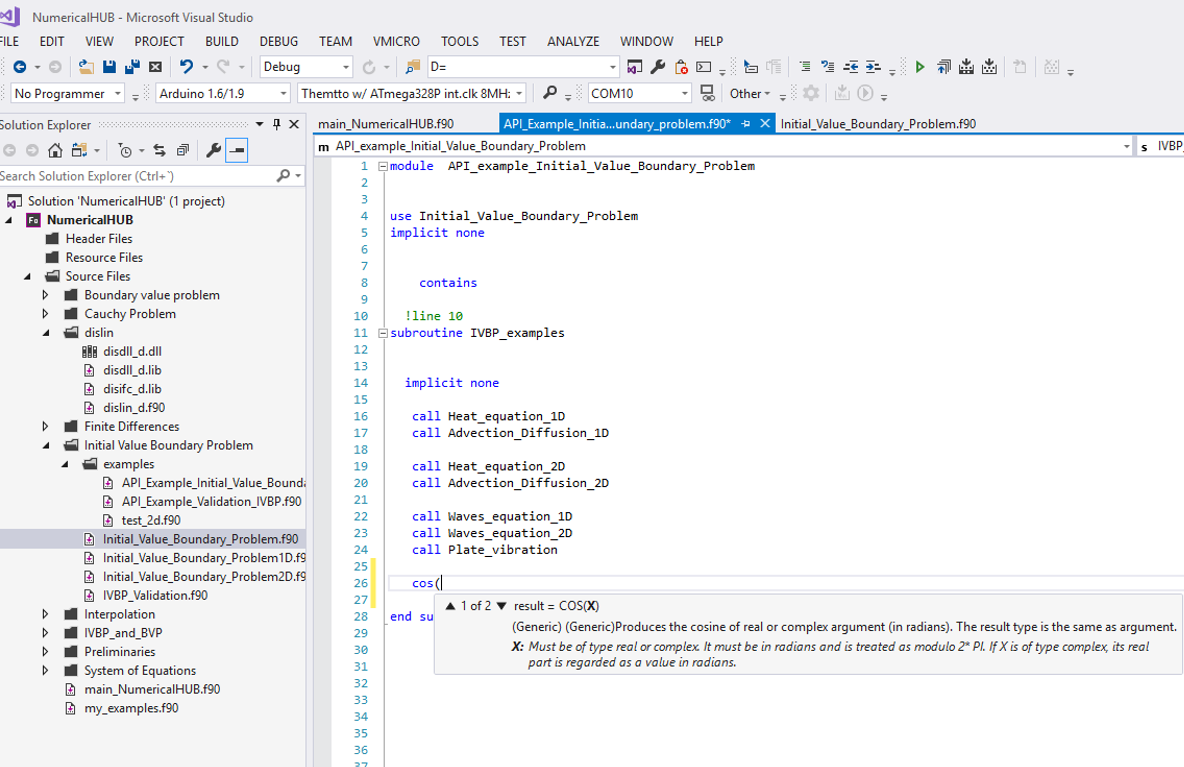
\includegraphics[width= \textwidth]{Figures/Commands5}
		\caption{Example of \textit{Intrinsic Parameter Info}.}
		\label{fig:Commands5}
	\end{figure}
	
	\begin{figure}
		\centering
		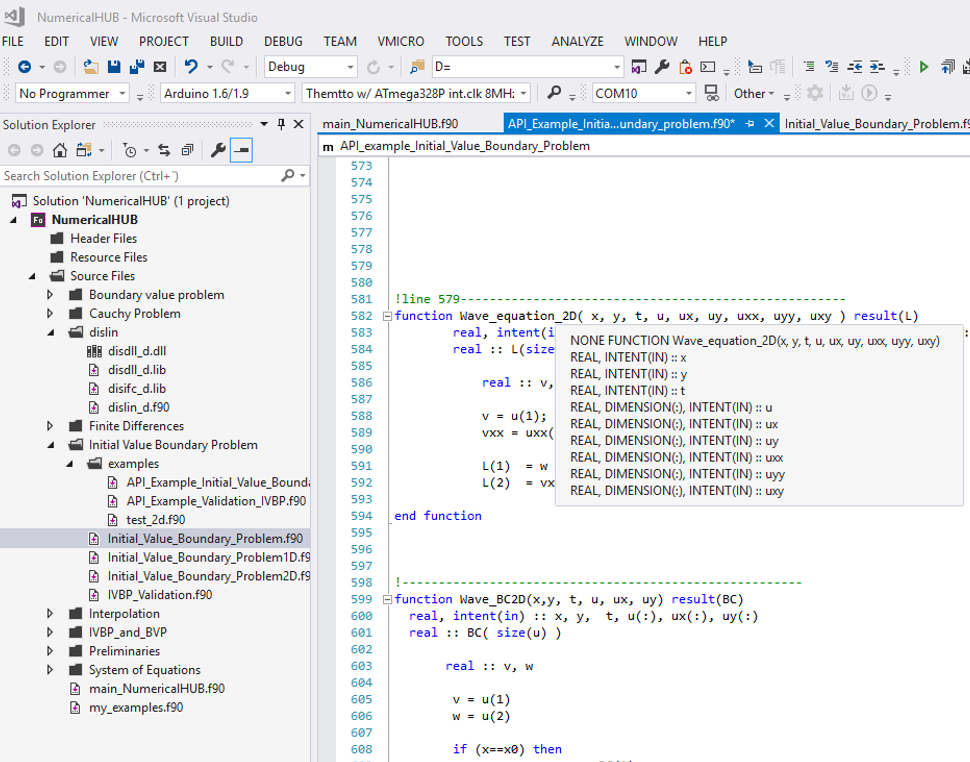
\includegraphics[width= \textwidth]{Figures/Commands6}
		\caption{Example of \textit{Intrinsic Quick Info}.}
		\label{fig:Commands6}
	\end{figure}
	
    
    \FloatBarrier
    %%%%%%%%%%%%%%%%%%%%%%%%%%%%%%%%%%%%%%%%%%%%%%%%%%%%%%%%%%%%%%%%%%%%%%%%%%%%%%%%%C
    \item \textbf{Executing the program: \textit{Start without Debugging}}
    
    This essential command of Visual Studio allows to \textbf{run the application/program} in all the different programming languages treated here. Once the program is written it can be executed by clicking on \textit{DEBUG/Start without Debugging}, pressing \textit{Ctrl+F5} or pressing the icon
    
    %\raisebox{-\mydepth}{\fbox{
\includegraphics[height=2\myheight]{Figures/StartSymbol}}}
    \begin{figure}[H]
        \centering
        
\includegraphics[width= 0.1\textwidth]{Figures/StartSymbol}
        %\caption{Example of \textit{Intrinsic Quick Info}.}
        %\label{fig:Commands6}
    \end{figure}
    
    of your toolbars. If you cannot see the mentioned icon in your toolbars take a look at the section \ref{sec:Shortcuts}.
    
    Notice that Visual Studio will launch your application without attaching the Debugger, you won't be able to pause the execution by breakpoints or use default debugging tools of the IDE. However, this is by far the most common method for executing programs in this guide. The behaviour of the command depends on the specific language used. For example, in Fortran it \textbf{saves} the modified files, \textbf{compiles}, \textbf{links} and \textbf{executes} all the project selected in the Solution Explorer. By contrast, in Python this command invokes the interpreter and the code is read and interpreted so the results can be shown in a command window.
    
    %%%%%%%%%%%%%%%%%%%%%%%%%%%%%%%%%%%%%%%%%%%%%%%%%%%%%%%%%%%%%%%%%%%%%%%%%%%%%%%%%C
    \item \textbf{Outlining blocks}
    
    \textbf{Outlining the source code} is one of the most common code folding patterns that IDEs and code editors offer. This feature allows to collapse a code block to a single line normally based on the syntax of the specific language used (other mechanisms appear depending on the indentation, the tokens or the preferences of the user). In general, the user can hide and show pieces of code that define a structure e.g. functions, subroutines, loops, if statements, etc. Then the code can be easily managed (specially if there is a large amount of text in the program) since only the headers of the hidden block are seen. Getting an overview of code and navigating through is now easier without being distracted by other code. The Figure \ref{fig:Outlining} shows an example.
    
    \begin{figure}
        \centering
        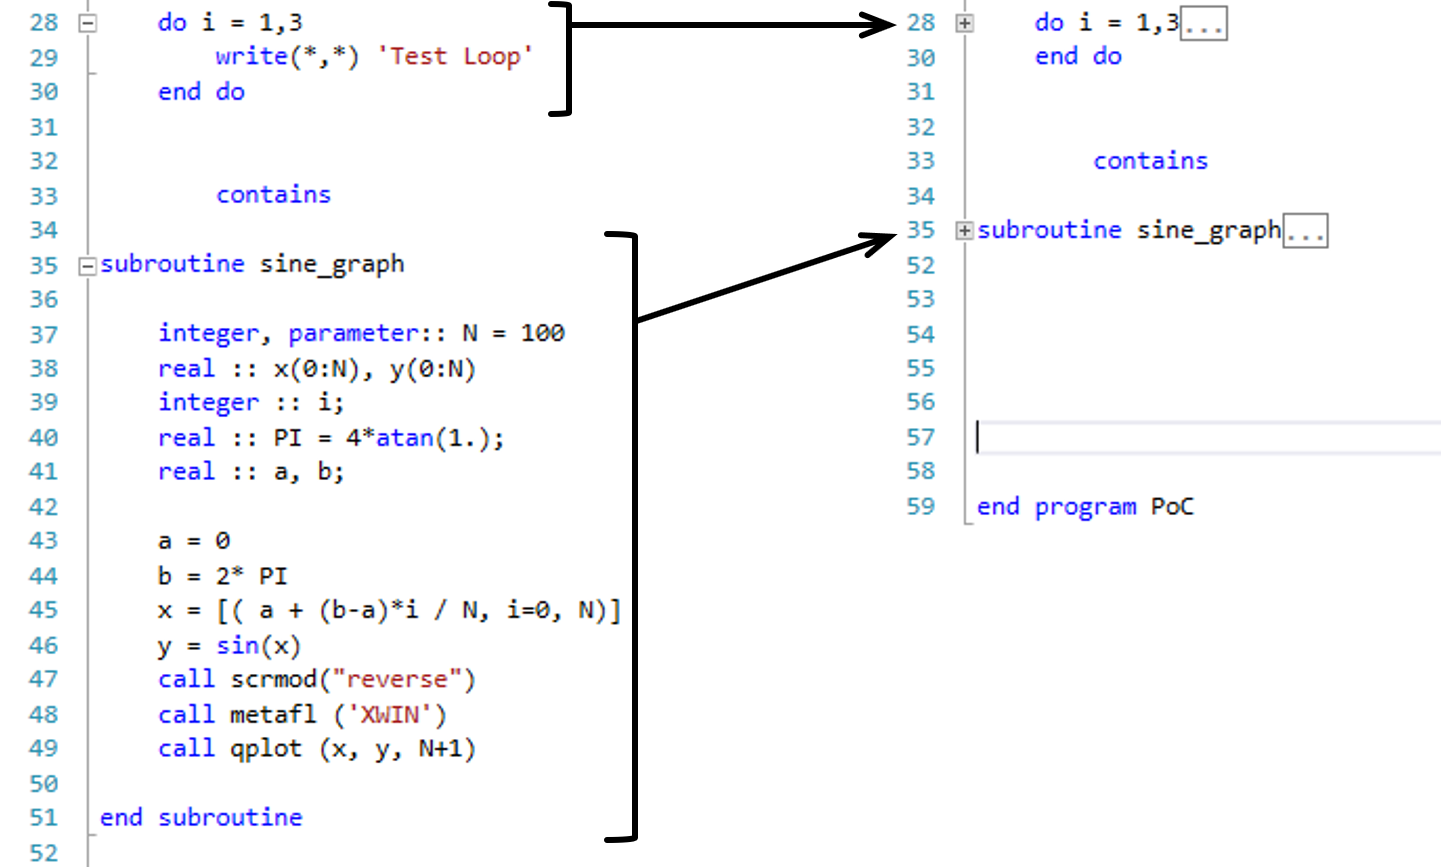
\includegraphics[width= \textwidth]{Figures/Outlining}
        \caption{Example of two pieces of code hidden by the user, one is a loop and the other a subroutine. By clicking on + or - we can deploy or hide the code.}
        \label{fig:Outlining}
    \end{figure}

    Depending on the language you are configuring the way to activate these features can vary, as an example we can go to \textit{TOOLS/Options.../Text Editor} and deploy the Fortran options. There click on \textit{Advanced} and in the menu called \textit{Outlining} mark \textit{True} in the options \textit{Enable Outlining} (which is actually activated by default) and \textit{Outline Statement Blocks} in case you also want to outline statements like loops. Notice that this options could be in a different menu for each programming language.
    
    If there is a piece of code where the outlining option does not appear automatically and you want to hide it, just do the following: select all the text to be outlined, right click on the selection, deploy \textit{Outlining} menu and click on \textit{Hide selection}. Then, that block of text can be shown and hidden on demand. 
    
    
    %%%%%%%%%%%%%%%%%%%%%%%%%%%%%%%%%%%%%%%%%%%%%%%%%%%%%%%%%%%%%%%%%%%%%%%%%%%%%%%%% 
    \item \textbf{Additional requirements}
    
    There are some tools that are common for a lot of Microsoft programs and in the case of the software development can be really useful. First of all, the different \textbf{extensions of the files} created in a software project are essential and the whole guide is full of references to some kind of files. Make sure that you have already activated in your Windows OS the option that shows the extensions of the files. If it is not activated, open any folder in your computer, click on \textit{View} and mark the option \textit{File name extensions}. From now on, you will see when a file is a C++ source code, a library or maybe a Fortran module.
    
    Part of the Visual Studio potential can be accessed using the \textbf{right button} of the mouse, exactly like the context menu of Windows OS. The options shown depend on the element where we deploy the pop-up menu and it is desirable to become familiarised with some commonly used functions. Just as an example, \textit{Go To Definition} and \textit{Find All References} will appear if we use the right button in the code (variables, calls to functions, intrinsic functions, etc.). If this button of the mouse is used in the solution explorer we can see different behaviour in the case of clicking on the name of projects and  the name of the solution. In the project the pop-up menu mainly shows the possibilities of Building, Rebuilding and Cleaning the project, adding folders or files and opening the properties of the project (which we will see in other chapters how important they are). However, in the name of the solution, the menu shows similar options but related to the whole solution (Build, Rebuild, Clean, Add existing or new projects, Rename the solution, open the solution properties, etc.). Try opening this menu in different places to get used to it.
    
    Exactly like in Windows OS we can make \textbf{bigger or smaller} what it is displayed in the screen, with the codes it is similar. Once you have your first piece of code opened in the IDE, try to make it bigger or smaller by pressing \texttt{Ctrl} and moving the scroll wheel of the mouse. The same effect could be achieved with the mouse pad.
    
    Finally, two different ways of \textbf{selecting pieces of code} can be used. The common way is pointing the cursor of the mouse in one line of the code, press \texttt{Ctrl+Shift} and click on a different part, all the lines between these two point will be selected. An useful alternative in order to select a vertical block of text is achieved by pressing the \texttt{Alt} key at the same time that the left button of the mouse and dragging the mouse in those lines we want to select.
    
    %%%%%%%%%%%%%%%%%%%%%%%%%%%%%%%%%%%%%%%%%%%%%%%%%%%%%%%%%%%%%%%%%%%%%%%%%%%%%%%%% 
    \item \textbf{Common IDE configuration}
    
    We can click on \textbf{\textit{Tools/Options...}} and start customizing the IDE in the \textbf{\textit{Environment}} menu. For example, the colour theme in the \textit{General} section (Dark, Light, Blue, etc.) or the auto-saving information frequency in the \textit{AutoRecover} tab can be decided here. We can also change the fonts and colours of the programming language or the default options for the \textit{Startup} (first window that appears when opening Visual Studio). 
    
    Since some compilers (e.g. GFortran) do not recognise tabs as characters, we could find warnings each time we compile a code with tabs instead of spaces. Hence, it is recommended to check that \textit{Insert Spaces} is marked in the \textit{Tabs} menu of the \textbf{\textit{Text Editor}} section (at least in the programming languages you are interested in).
    
    %%%%%%%%%%%%%%%%%%%%%%%%%%%%%%%%%%%%%%%%%%%%%%%%%%%%%%%%%%%%%%%%%%%%%%%%%%%%%%%%% 
    \item \textbf{Windows inside the IDE}
    
    Related to the different \textbf{windows} around the environment, the behaviour is the same as Windows OS. We can change position, make them fixed or floating, configure different options, etc. We can decide for each window in a little arrow located in the right upper part, also close those we do not need or open new ones in \textbf{\textit{View}} tab. \textit{Solution Explorer}, \textit{Properties Window}, \textit{Bookmark Window} or \textit{Output} are some windows we are going to need from now on. The Figure \ref{fig:Config1} shows an example of distribution of two essential windows: \textbf{Solution Explorer} and \textbf{Output}, we can choose our favourite position and move them. If we want to move the windows we grab it and Visual Studio will show us some default positions we could choose, we just have to drop it in the little boxes shown (or drop it in a floating point).
    
    \begin{figure}
        \centering
        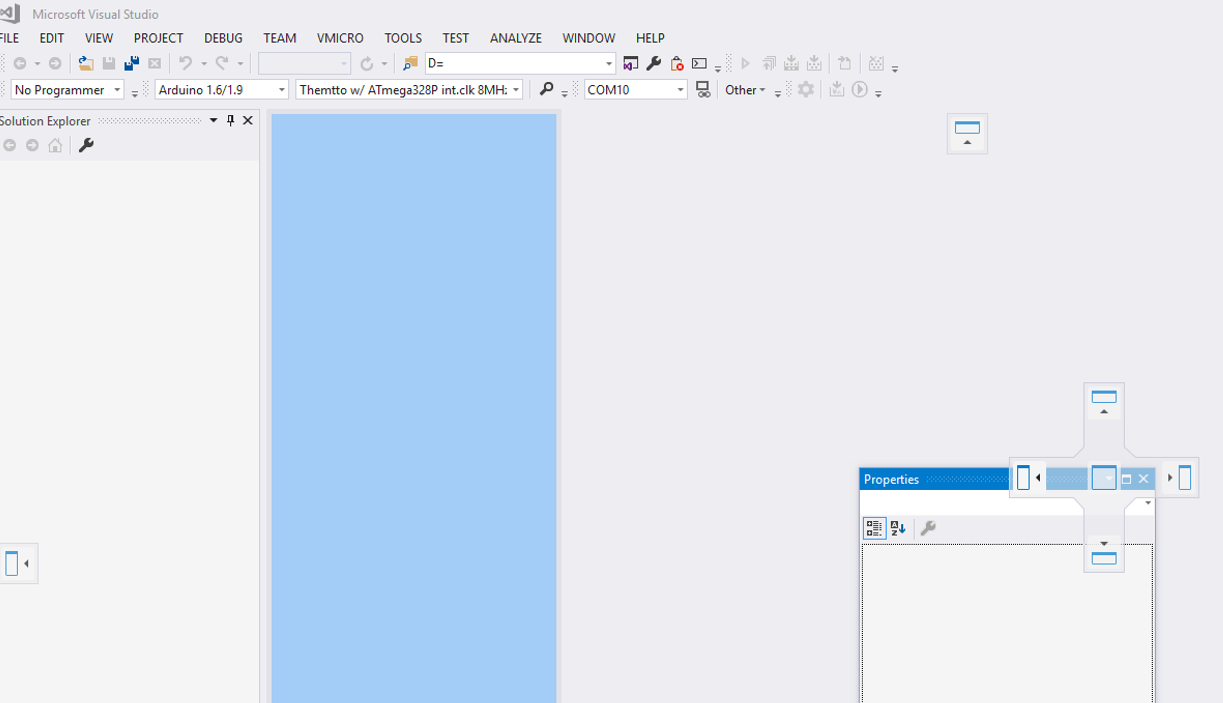
\includegraphics[width= \textwidth]{Figures/Config1}
        \caption{Example of windows distribution with a Fortran project already opened, \textit{Solution Explorer} and \textit{Output} windows are going to be intensively used.}
        \label{fig:Config1}
    \end{figure}

    \newpage
    %%%%%%%%%%%%%%%%%%%%%%%%%%%%%%%%%%%%%%%%%%%%%%%%%%%%%%%%%%%%%%%%%%%%%%%%%%%%%%%%%C
    \item \textbf{Find in Files, Find and Replace} \label{list:FIND}
    
    \textit{Find in Files} is a powerful Visual Studio feature that allows to search in a set of files terms. It can look for the term in the entire solution, only in the opened document, in the opened project, etc. This feature is complemented by the tool \textit{Replace in Files} which can automatically replace all the terms of a project or document by another term. Both tools can be found in the same window: \textit{Find and Replace}. 
    
    Open the window by clicking on \textit{Edit/Find and Replace/Find in Files}, it will be shown at the right part of the IDE by default. Then you can change the position of the window, hide it temporally (with the option of showing it quickly), make it floating or close it, all can be done with the symbols in the top-right part of the window. Once you have the tool opened, change between both features and write a term to look for or replace. The results of the search will appear in the \textit{Find Results} window, which is automatically opened, then it is possible to navigate through the different results in the code itself by pressing \textit{Find previous} and \textit{Find Next}. 
    
    It is a commonly used feature in the IDE so we recommend to maintain the window accessible in the environment. It is treated how to show new commands and toolbars in the section \ref{sec:Shortcuts}. Take a look at the Figure \ref{fig:Config4-2} and check the symbol of the tool \textit{Find in Files}. In addition, \textit{Go To Find Combo} bar is shown in the same toolbar and both icons have to be activated since they are not shown by default.
  

\end{enumerate}


    \vspace{-0.5cm}
    \FloatBarrier
    \section{Importing the environment configuration}
    
This manual is accompanied by a settings file called \texttt{Exported-2019-07-03.vssettings} (or updated name) which makes automatically all the changes explained in this guide. Open this url to download the file:

\url{https://github.com/jahrWork/Visual-Studio-projects}
 
We can import this configuration and then all the options treated will be automatically applied. Go to \textit{Tools/Import and Export Settings/Import selected environment settings} and click on \textit{Next}, in the next window decide if creating or not a backup of your actual configuration, depending on your needs. Click on \textit{Next} again and then in \textit{Browse}, look for the file downloaded from the Git repository and open it. Finally click on \textit{Next} and \textit{Finish}.    
    
If you change the configuration of the environment it is interesting to make a \textbf{backup copy} of the configuration in order to restore it easily if you reinstall Visual Studio, work in two different computers or change your personal computer. Go to \textit{Tools/Import and Export Settings/Export selected environment settings}, click on \textit{Next} twice and choose where to save it.
    
\begin{IN}
    \begin{itemize}
        \item Please notice that the file \texttt{Exported-2019-07-03.vssettings} (or similar name) that comes with this manual only stores the \textbf{IDE configuration} and not the preferences and options related to the project configurations of the different programming languages.
            
        \item It is also important to notice that the configuration file could keep \textbf{sensitive information}, which means that maybe some options store links to folders in the computer where the configuration was made and exported. In this case, when the IDE follows the links an error message appears and you must change the link to the corresponding folder in your computer. This can also happen when you create your own configuration files and use it in more than one computer.  
    \end{itemize}
\end{IN}
    

    \section{Modifying shortcut icons} \label{sec:Shortcuts}

The Figure \ref{fig:Commands} shows some commands that are going to be highly used when programming so we recommend to enable the quick access in the toolbars. The first two of them comment and uncomment the code selected and next two decrease and increase the indentation. The fifth one is the \textit{Start without Debugging} button (already explained) and the last active buttons are in charge of compiling and building our program. While the first compiles the current file, the second builds the project or library selected and the last builds the whole solution (which we know can contain more than one project). These functionalities will be explained in the chapters of the different programming languages. 

\begin{figure}[h]
    \centering
    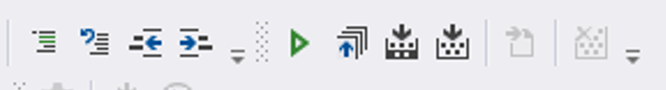
\includegraphics[width= 0.9 \textwidth]{Figures/Commands}
    \caption{Very useful commands when programming, it is advisable to show them in the toolbars.}
    \label{fig:Commands}
\end{figure}

\vspace{0.5cm}
We can personalise all the \textbf{toolbars} and \textbf{commands} that the IDE shows and it can be done in two ways. Firstly, by clicking on the right part of each toolbar we see the option \textit{Add or Remove Buttons} which deploys a list of default options for that bar (Figure \ref{fig:Config2}). Secondly, we can click on \textit{Tools/Customize} and we access two tabs: \textit{Toolbars} (Figure \ref{fig:Config3}), which can show and hide a big list of toolbars and \textit{Commands} where we can select any of them, add and delete commands and also add new buttons that are not in the bar by default (figures \ref{fig:Config4-2}, \ref{fig:Config4} and \ref{fig:Config4-3}). 

In these mentioned figures we can see that the \textit{Text Editor}, \textit{Standard}, \textit{Build} and \textit{Micro} toolbars are shown. The Figure \ref{fig:Config4-2} shows that \textit{Standard} bar includes new commands like \textit{Find in Files}, \textit{Solution Explorer} and \textit{Properties Window} while \textit{Build} bar (figure \ref{fig:Config4}) includes \textit{Compile} command and the most important; \textbf{\textit{Start without debugging}}.\label{StartwD} It is necessary to have quick access to this command because most of the times we won't use the default debugger and we just want to run the code directly without debugging. Finally, the toolbar \textit{Text Editor} (figure \ref{fig:Config4-3}) is really useful while writing code because of the \textit{Comment} and \textit{Uncomment} commands or the new ones added, \textit{Line Indent} and \textit{Line Unindent}. We should take the time to organize buttons and include those we use more. 

\begin{figure}[h]
    \centering
    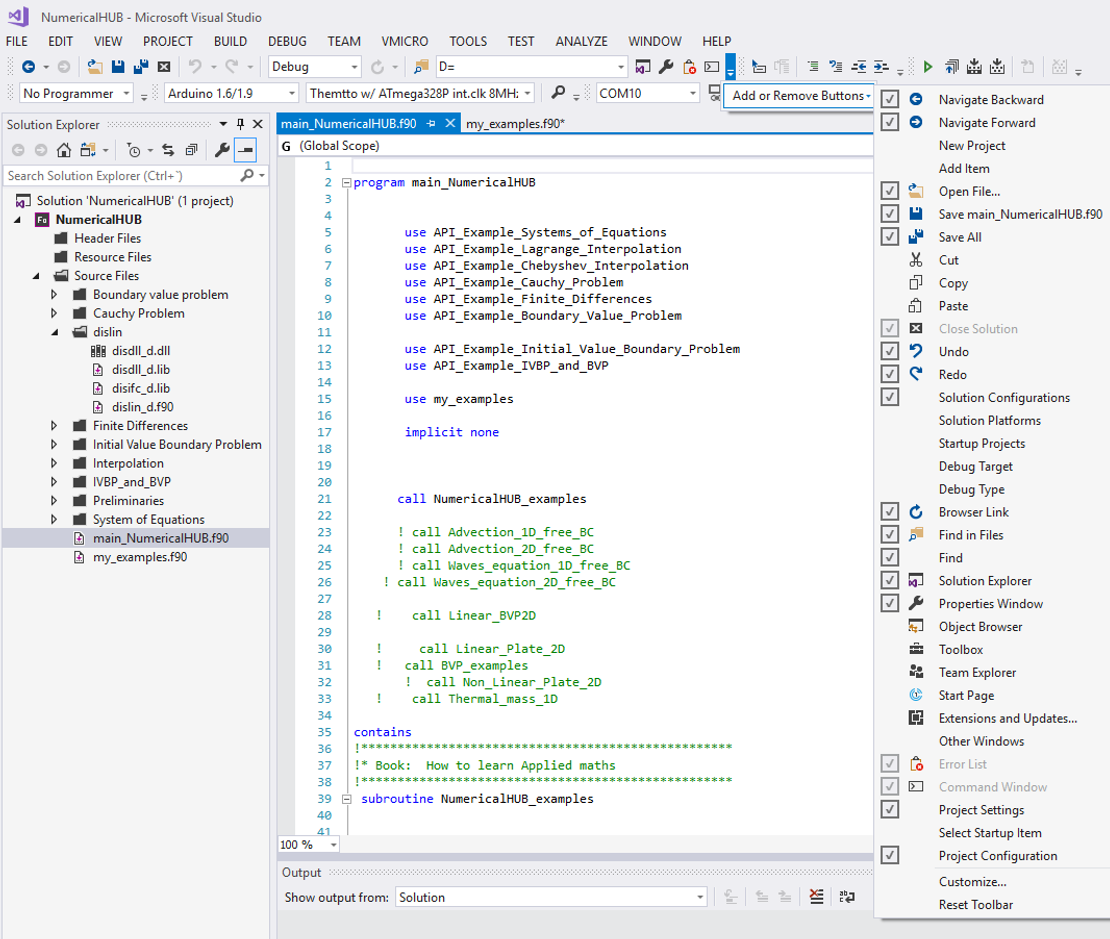
\includegraphics[width=\textwidth]{Figures/Config2}
    \caption{Add and Remove options for the buttons that appear in the toolbars.}
    \label{fig:Config2}
\end{figure}

\begin{figure}[h]
    \centering
    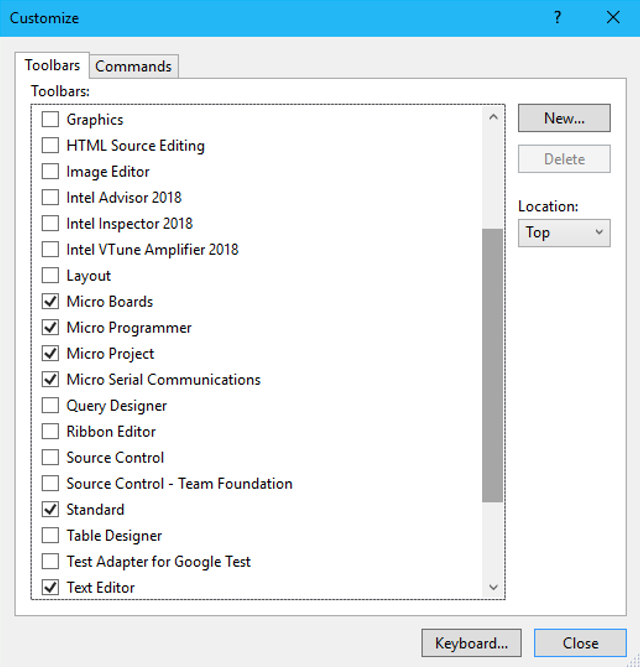
\includegraphics[width= \textwidth]{Figures/Config3}
    \caption{\textit{Toolbars} tab in the menu \textit{Tools/Customize}, it allows to show and hide toolbars for the IDE.}
    \label{fig:Config3}
\end{figure}

\begin{figure}[h]
    \centering
    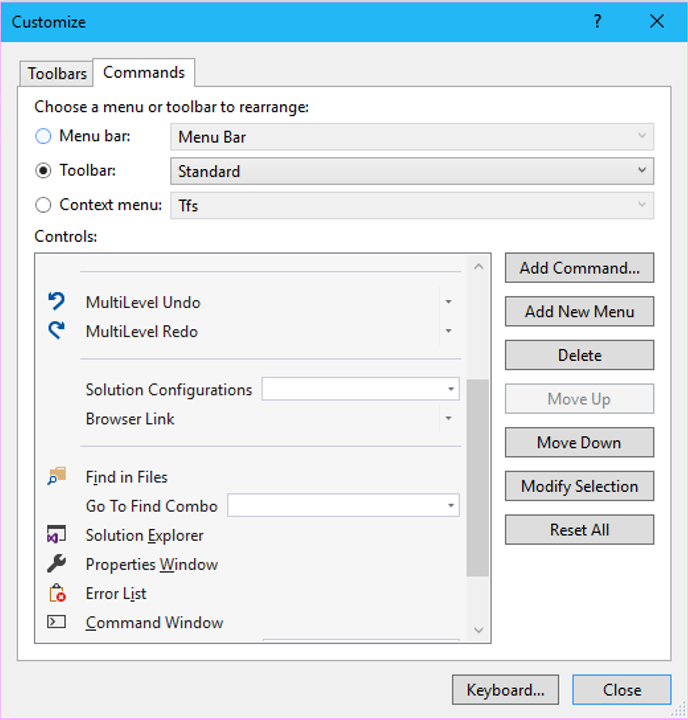
\includegraphics[width= 0.6\textwidth]{Figures/Config4-2}
    \caption{\textit{Commands} tab in the menu \textit{Tools/Customize}, it adds commands to the selected toolbar or menu, in this case the \textit{Standard} Toolbar.}
    \label{fig:Config4-2}
\end{figure}

\begin{figure}[h]
    \centering
    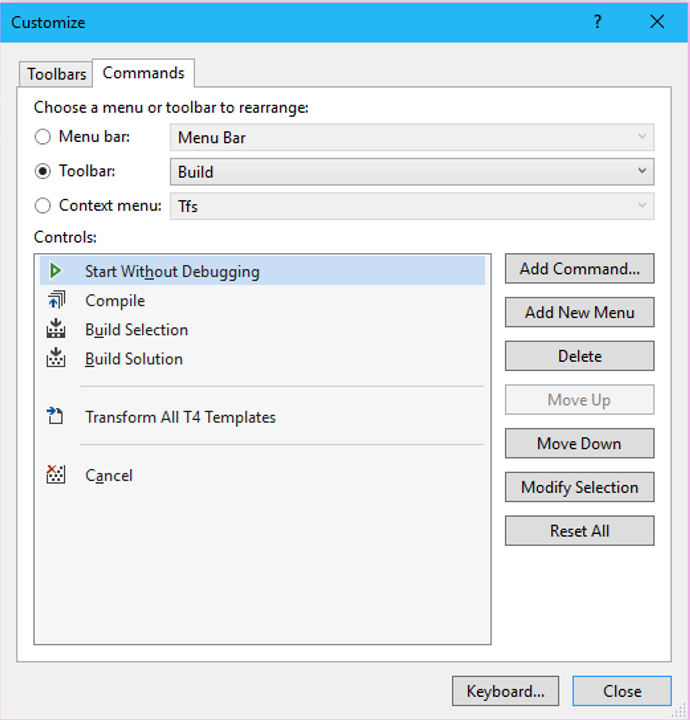
\includegraphics[width= 0.6\textwidth]{Figures/Config4}
    \caption{\textit{Commands} tab in the menu \textit{Tools/Customize}, it adds commands to the selected toolbar or menu, in this case the \textit{Build} Toolbar.}
    \label{fig:Config4}
\end{figure}

\begin{figure}[h]
    \centering
    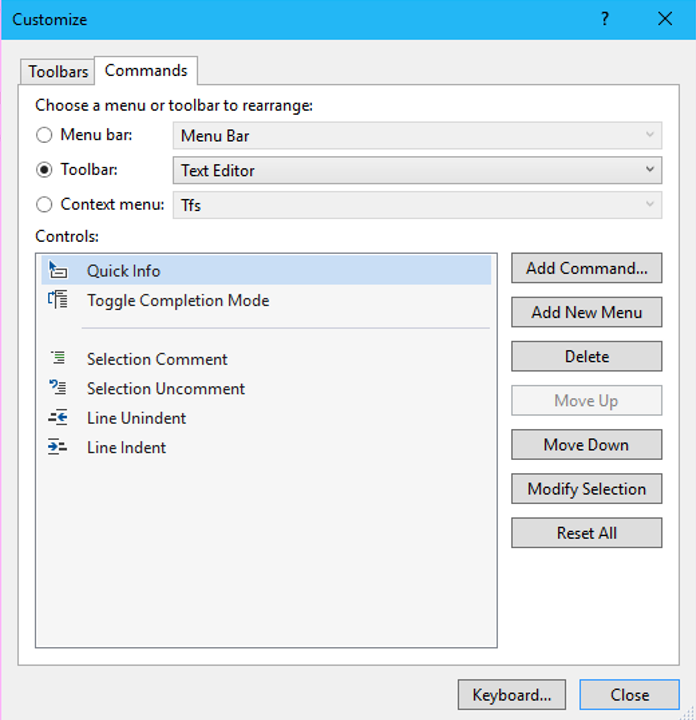
\includegraphics[width= \textwidth]{Figures/Config4-3}
    \caption{\textit{Commands} tab in the menu \textit{Tools/Customize}, it adds commands to the selected toolbar or menu, in this case the \textit{Text Editor} Toolbar.}
    \label{fig:Config4-3}
\end{figure}
    

    
    
    

    \FloatBarrier
    \section{Enterprise distribution of Visual Studio} \label{sec:Enterprise}

If you are interested in the Enterprise distribution of Visual Studio you can download the installer from the same webpage used for the Community version (\url{https://visualstudio.microsoft.com/es/downloads/}) or follow all the steps mentioned below. In this case you need an academic license to activate the product. We are going to see how to obtain that license using \textit{Azure Dev Tools for Teaching}, a Microsoft repository created for university departments and students.

Obtaining an academic license and the installer for Visual Studio Enterprise. 

\begin{enumerate}
    \item Click directly on (Figure \ref{fig:ExtraA}):
    
     \url{https://azureforeducation.microsoft.com/devtools}
    \item Click on the blue button \textit{Sign In} and Initiate session using your institutional email (finished with \textit{@alumnos.upm.es}, Figure \ref{fig:ExtraB}).
    \item You will be redirected to the authentication service of the UPM. Write your email once again and write the password for that email account (Figure \ref{fig:ExtraC}).
    \item After accepting a message that allows you to maintain the session opened, you access the Microsoft Azure environment with the tab \textit{Education} shown (Figure \ref{fig:ExtraD}).
    \item There, you may see the last release of Visual Studio in the right part of the window. However, you can also click on \textit{Software}, look for \textit{Visual Studio Enterprise} in the list or write it in the search bar.
    \item Click on the name of the tool and you will have access to the download of the installer and the Key for activating the product (Figure \ref{fig:ExtraE}). 
    \item Download the installer for the Enterprise distribution and keep safe the Key, you are going to use it later.    
\end{enumerate}

\begin{figure}
    \centering
    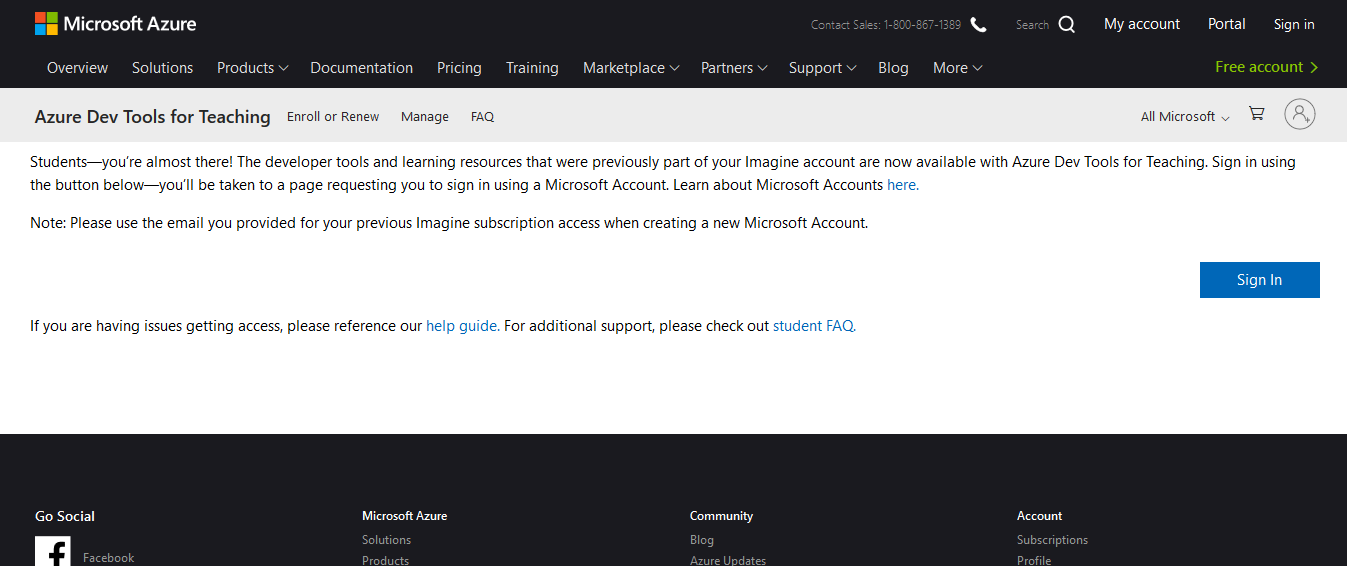
\includegraphics[width= \textwidth]{Figures/ExtraA}
    \caption{Main webpage of Microsoft Azure Dev Tools for Teaching where we have to click on \textit{Sign In}.}
    \label{fig:ExtraA}
\end{figure}

\begin{figure}
    \centering
    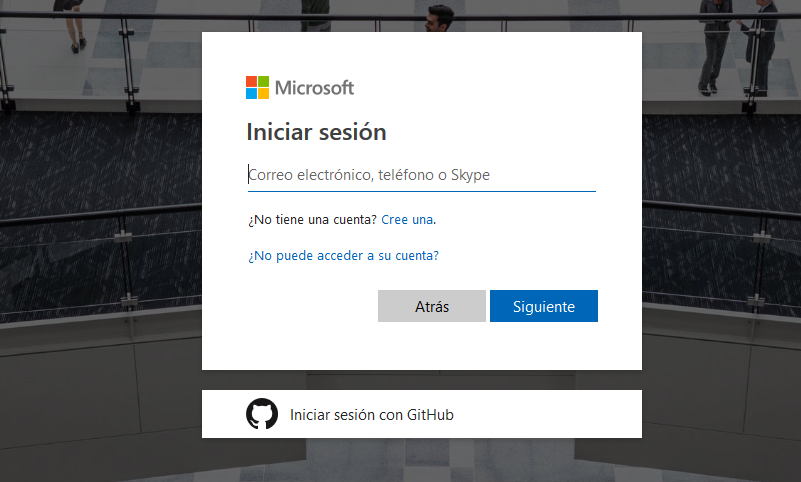
\includegraphics[width= \textwidth]{Figures/ExtraB}
    \caption{Start session window, the institutional email must be used here (finished with @alumnos.upm.es).}
    \label{fig:ExtraB}
\end{figure}

\begin{figure}
    \centering
    
\includegraphics[width= \textwidth]{Figures/ExtraC}
    \caption{Authentication service of the UPM, you must use your institutional email and the same password used in the email account.}
    \label{fig:ExtraC}
\end{figure}

\begin{figure}
    \centering
    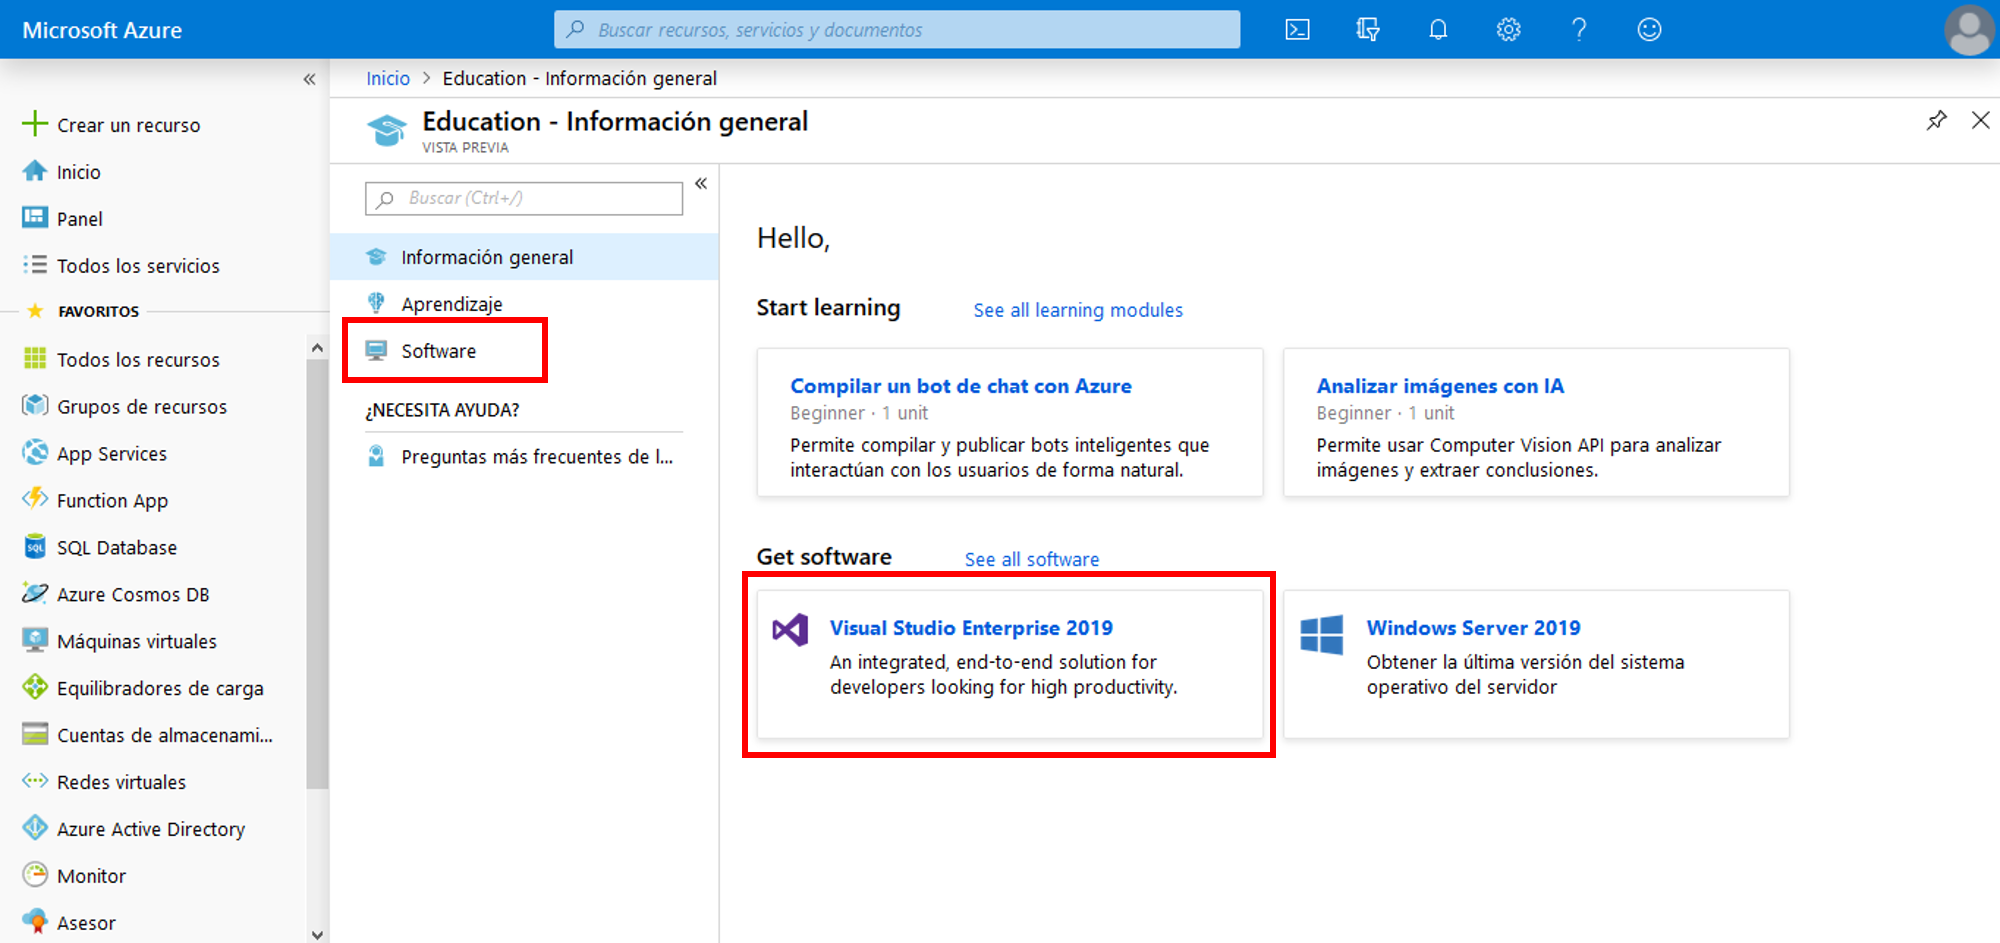
\includegraphics[width= \textwidth]{Figures/ExtraD}
    \caption{Start window of Microsoft Azure, Visual Studio Enterprise is already shown but we could look for it in the \textit{Software} space if needed.}
    \label{fig:ExtraD}
\end{figure}

\begin{figure}
    \centering
    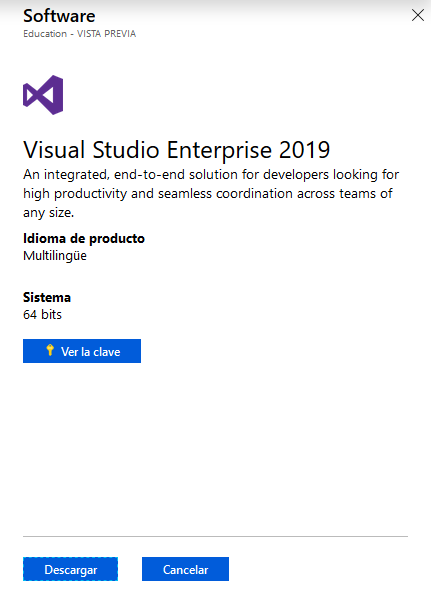
\includegraphics[width= 0.6 \textwidth]{Figures/ExtraE}
    \caption{Menu where we can download the installer of Visual Studio Enterprise and consult the key used to activate the tool.}
    \label{fig:ExtraE}
\end{figure}

In order to install Visual Studio Enterprise version with an academic license in Windows you can follow the same process seen in the installation of the Community version, executing this time the installer of the Enterprise version. The name now is similar to \texttt{vs\_enterprise\_xxxxx.exe}. As a difference, in the step 7 you have to activate the product using your Key:

\begin{enumerate}
    \setcounter{enumi}{6}
    \item Notice that in the top right part of the IDE it is shown that you have already started session. If you click on the letter of your name and \textit{Account Configuration} (see figure \ref{fig:Instalacion3}) you will see that your credentials are activated. In the right part of that window it may say that you are using a 30 days license, click on \textit{Unlock with a Product Key} (see figure \ref{fig:Instalacion5}) and it will show a window waiting for the Key obtained (see figure \ref{fig:Instalacion6}). Click on \textit{Apply} and the message ``Product Key applied'' should appear. 
    \item Your IDE is ready to work now. 
\end{enumerate}

\begin{figure}
    \centering
    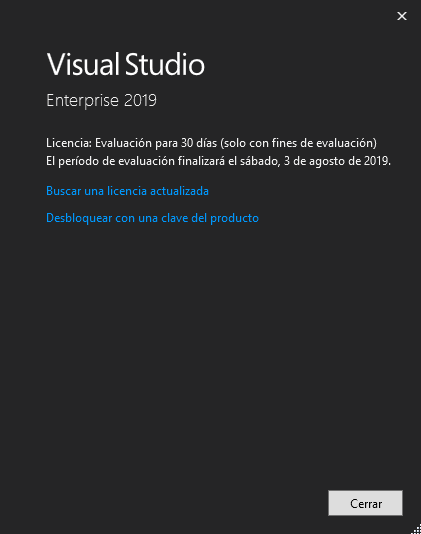
\includegraphics[width= 0.7\textwidth]{Figures/Instalacion5}
    \caption{License information in the Account Configuration window in the IDE, before activating the product you will have a 30 days license.}
    \label{fig:Instalacion5}
\end{figure}

\begin{figure}
    \centering
    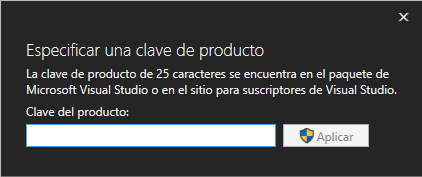
\includegraphics[width= 0.6\textwidth]{Figures/Instalacion6}
    \caption{Activation window, copy here the key obtained with \textit{Azure Dev Tools for Teaching} and click on \textit{Apply}.}
    \label{fig:Instalacion6}
\end{figure}



%------------------------------------------------------------------------------------------------------------------------------------------------------
%------------------------------------------------------------------------------------------------------------------------------------------------------
%As an example, we are going to see how to download Visual Studio with academic license using \textit{OnTheHub}, a repository where essential tools of the industry are offered to the universities.
%
%\begin{enumerate}
%    \item We click directly on this url; \url{http://e5.onthehub.com/WebStore/ProductsByMajorVersionList.aspx?ws=f1b11fc4-826f-e011-971f-0030487d8897&vsro=8&JSEnabled=1}.
%    \item Log in here (top right part of the window) using our institutional email (finished with \textit{@alumnos.upm.es}) and enter with same password as our personal account (figure \ref{fig:Proceso1}).
%    \item In the search line we write ``Visual Studio Enterprise 2017''. The first result that appears is our IDE, we click on \textit{Add to cart} and go to the Shopping Cart.
%    \item Follow the instructions shown. We will be asked for the name, surname and email for confirming the process (Figure \ref{fig:Proceso2} and \ref{fig:Proceso3}).
%    \item Once we complete the information, the details of the purchase appear with the Order Number and the License Key (an email with the purchase details is also sent to our account). Figure \ref{fig:Proceso4} shows the download button. Do not forget to store the License Key and the Order Number for future requests. 
%    \item Click on \textit{Download}. The file \textit{vs\_enterprise\_xxxxx.exe} should be downloaded in your downloads folder.      
%\end{enumerate}
%
%\begin{figure}
%    \centering
%    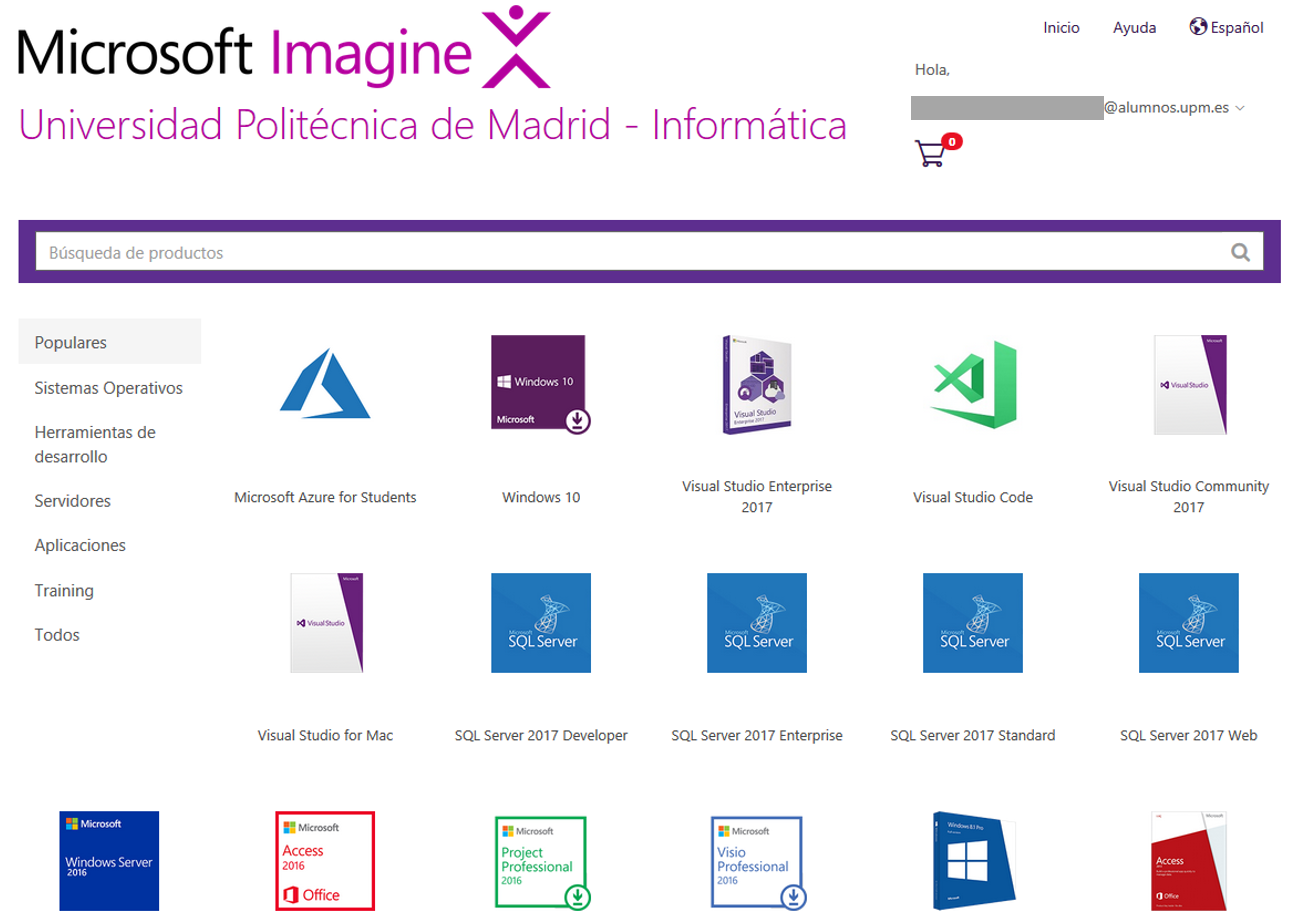
\includegraphics[width= \textwidth]{Figures/Proceso1}
%    \caption{Home page of the software repository of Microsoft, we log in and search for Visual Studio 2017.}
%    \label{fig:Proceso1}
%\end{figure}
%
%\begin{figure}
%    \centering
%    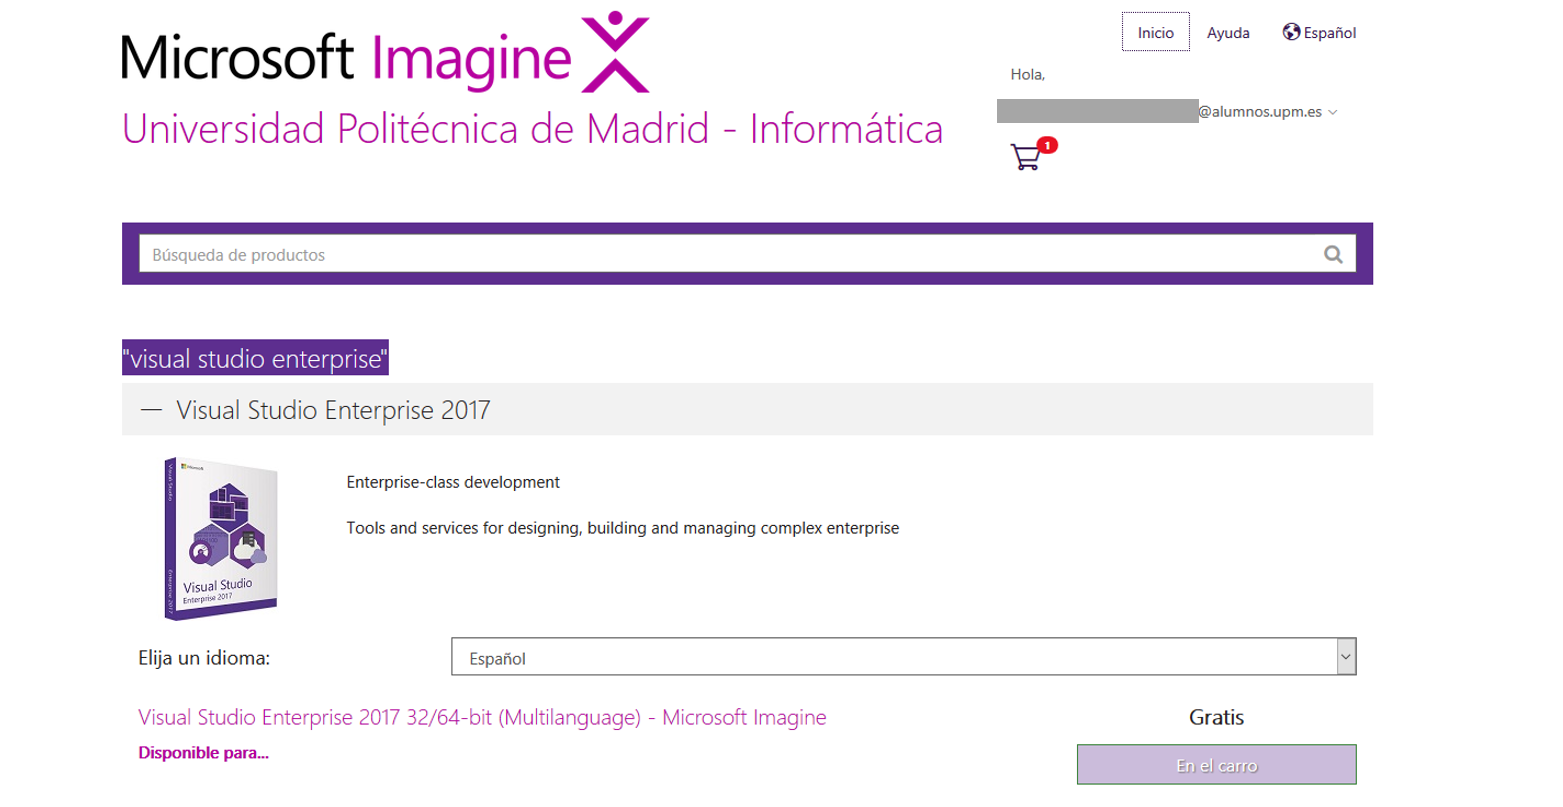
\includegraphics[width= \textwidth]{Figures/Proceso2}
%    \caption{Version of Visual Studio chosen, Enterprise 2017. We have to write name, surname and email.}
%    \label{fig:Proceso2}
%\end{figure}
%
%\begin{figure}
%    \centering
%    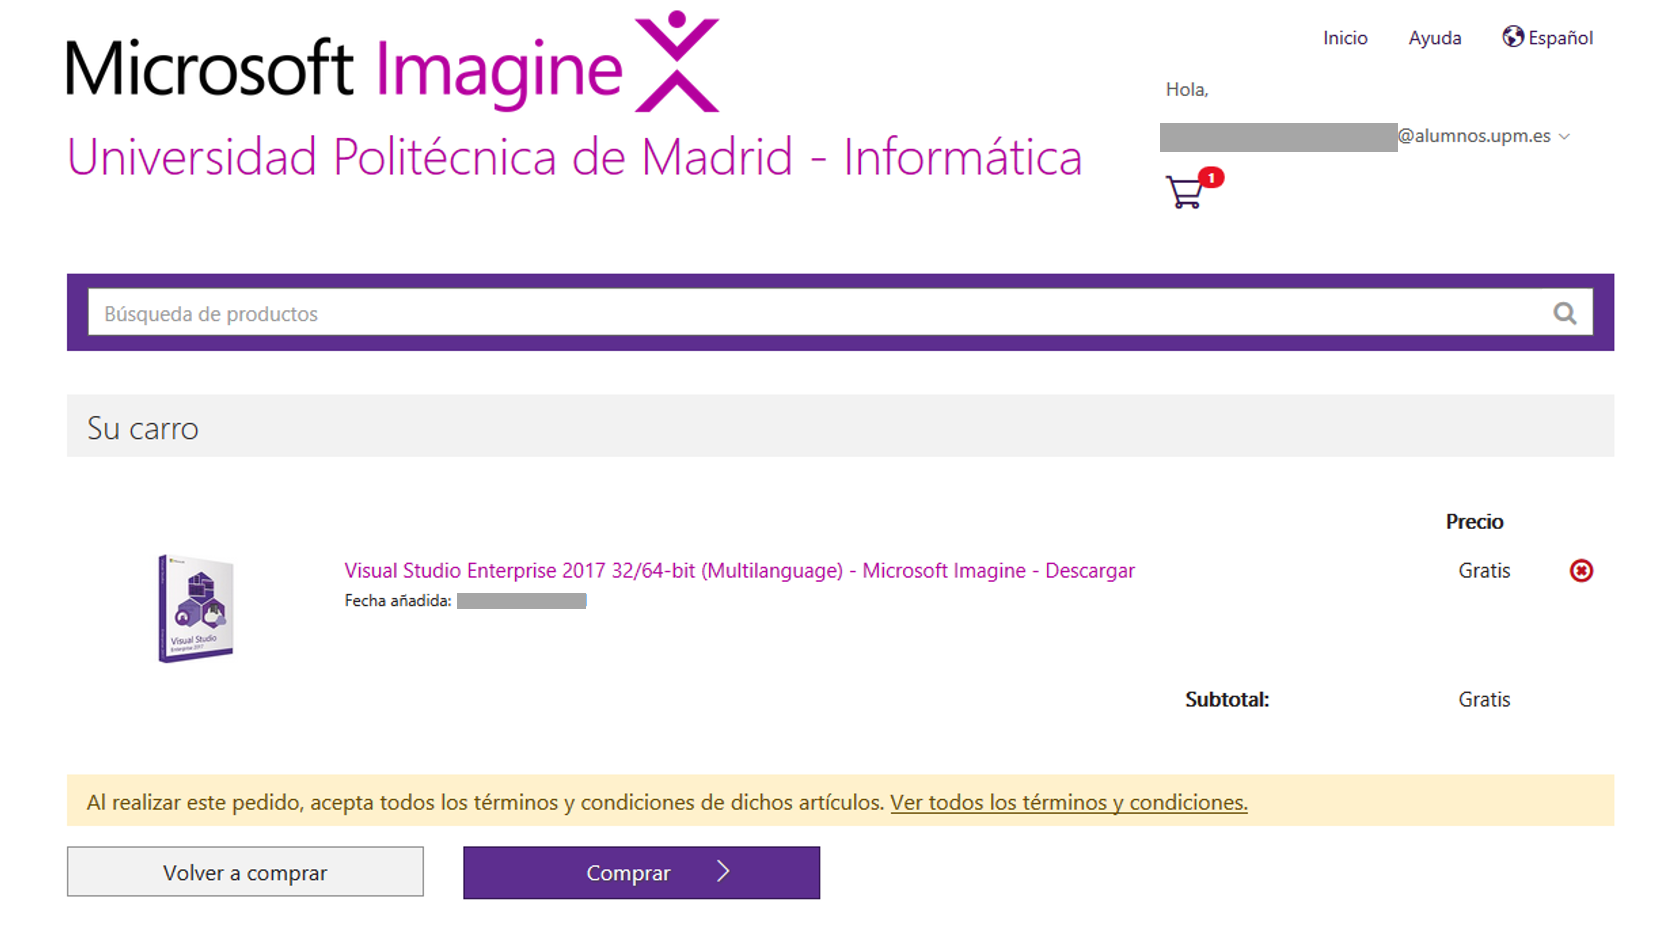
\includegraphics[width= \textwidth]{Figures/Proceso3}
%    \caption{Shopping Cart with Visual Studio Enterprise 2017 chosen.}
%    \label{fig:Proceso3}
%\end{figure}
%
%\begin{figure}
%    \centering
%    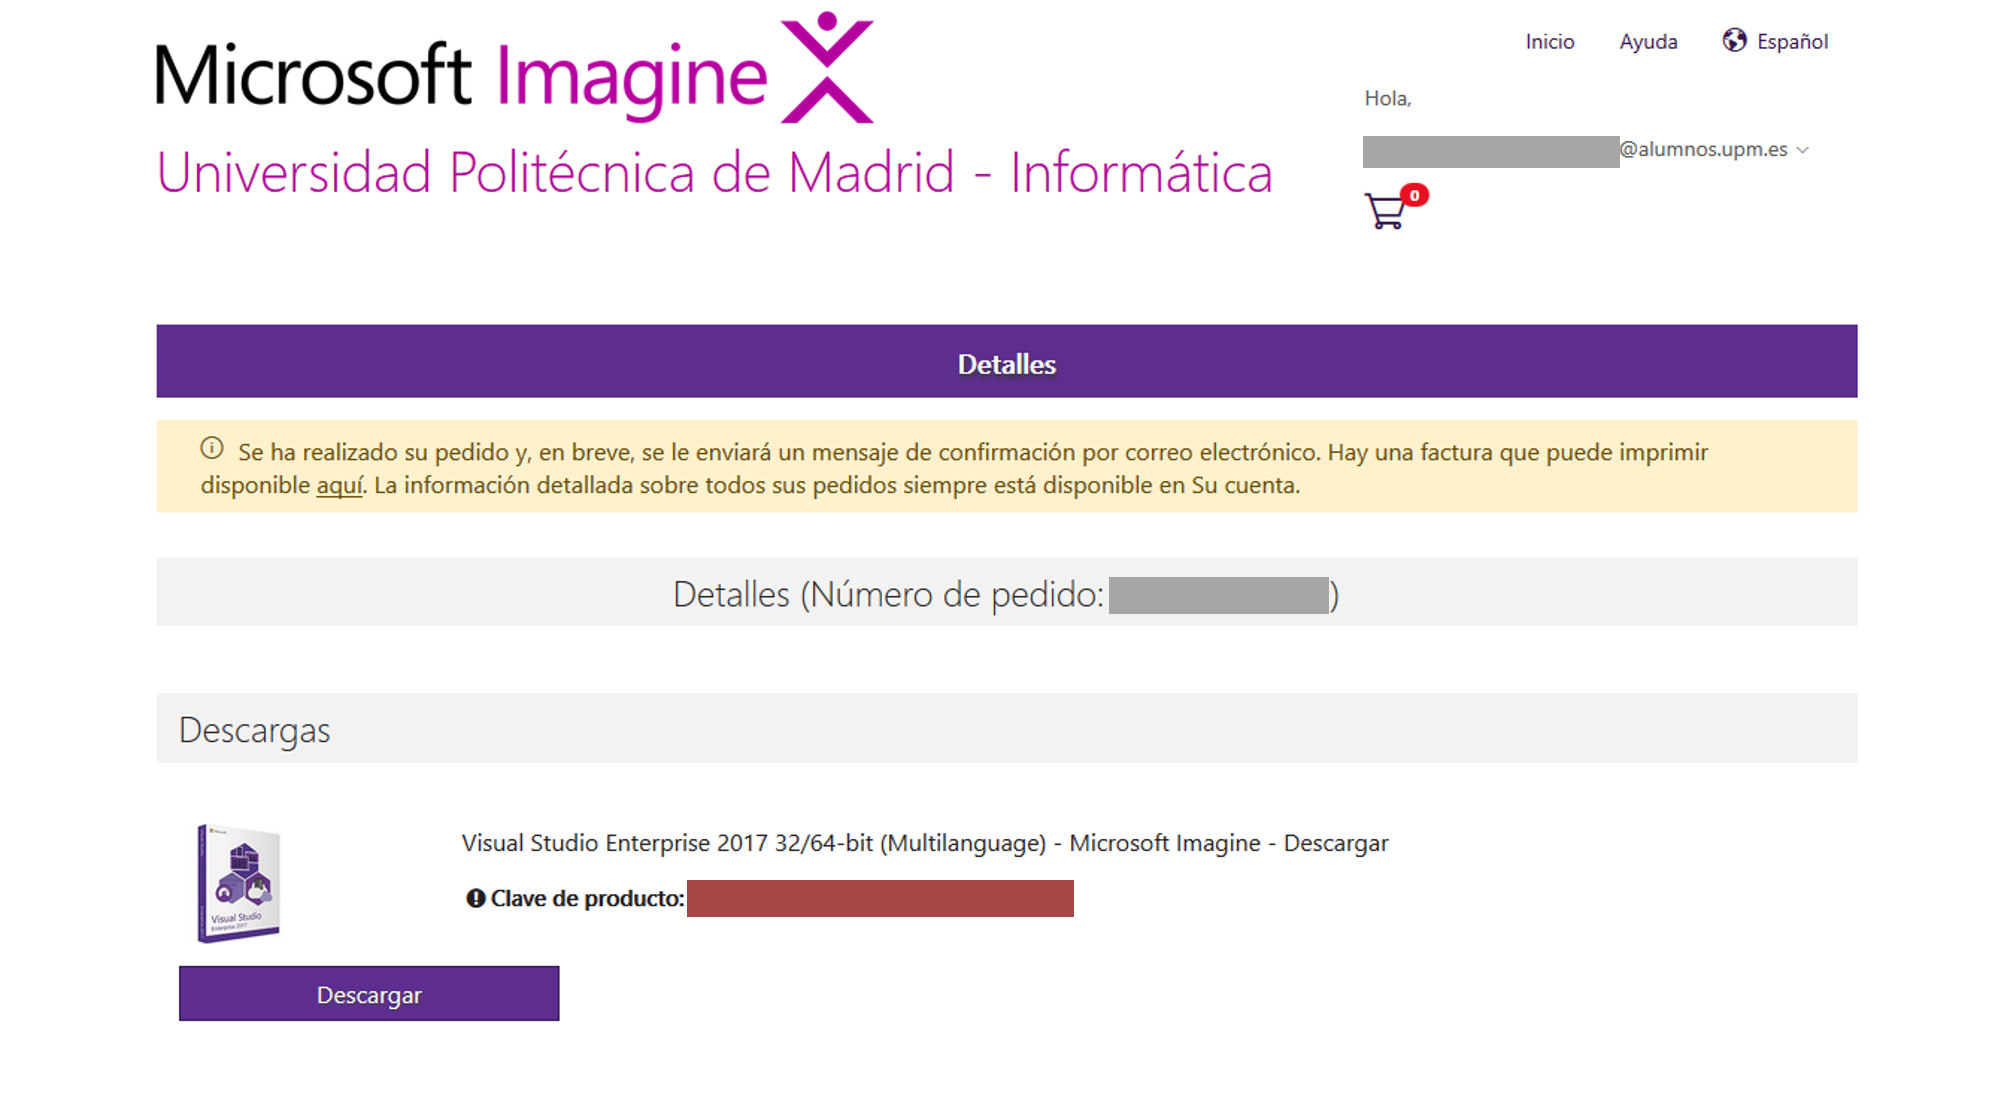
\includegraphics[width=  \textwidth]{Figures/Proceso4}
%    \caption{Details of our License Key and Order Number, we should save this information.}
%    \label{fig:Proceso4}
%\end{figure}
%------------------------------------------------------------------------------------------------------------------------------------------------------
%------------------------------------------------------------------------------------------------------------------------------------------------------


